% =====================================================================
% main-zh.tex -- LINGSHU 中文版（单独成篇，XeLaTeX）
% 内容：sections-zh/ 下的中文全文；英文版仍以 main.tex 为 source of truth。
% 交叉引用：中文文件不含 \label，通过 xr 从英文编译产物（../en/main.aux）导入编号。
% 构建：先构建英文（rebuild.ps1 en），再 xelatex main-zh ×3。
% =====================================================================
\documentclass[11pt]{article}

\usepackage[a4paper,margin=0.9in]{geometry}
\usepackage{fontspec}
\usepackage{xeCJK}
\setmainfont{Times New Roman}
\setCJKmainfont[Path=C:/Windows/Fonts/, Extension=.ttf]{simhei}
\setCJKmonofont[Path=C:/Windows/Fonts/, Extension=.ttf]{simhei}
\usepackage{amsmath}
\usepackage{amssymb}
\usepackage{booktabs}
\usepackage{graphicx}
\usepackage{microtype}
\usepackage[numbers,sort&compress]{natbib}
\usepackage[colorlinks=true,linkcolor=black,citecolor=blue,urlcolor=blue]{hyperref}
\usepackage{url}
\usepackage{seqsplit}
\usepackage{listings}
\lstset{basicstyle=\ttfamily\footnotesize,breaklines=true,columns=fullflexible,
  keepspaces=true,frame=none,aboveskip=4pt,belowskip=4pt}

% 从英文版 aux 导入 label 编号（中文版本身不定义 label）
\usepackage{xr}
\externaldocument{../en/main-en}

\setlength{\parskip}{2pt}
\frenchspacing
\renewcommand{\arraystretch}{1.3}
\sloppy
\setlength{\emergencystretch}{2em}

% 中文版的固定名称（标题、图表、参考文献、附录）
\renewcommand{\figurename}{图}
\renewcommand{\tablename}{表}
\renewcommand{\refname}{参考文献}
\renewcommand{\appendixname}{附录}
\renewcommand{\abstractname}{摘要}
\renewcommand{\contentsname}{目录}

\newcommand{\system}{\textsc{LingShu}}
\newcommand{\host}{\textsc{Dsh}}

\title{灵枢：面向 Agent 宿主可审计认知插件的\\控制论控制面\\[6pt]
\large 预印本初稿 · 中文版\\[2pt]
\normalsize\itshape LINGSHU: A Cybernetic Control Plane for Auditable Cognition Plugins in Agent Hosts}
\author{\system{} Project Team}
\date{2026 年 10 月}

\begin{document}
\maketitle

\noindent\textbf{说明。} 本文件是论文的中文版，内容与英文版（\texttt{main.tex}）逐节对应；若中英出现歧义，以英文版为准。数值、限定词与边界声明均与英文版一致。

\begingroup
\renewcommand{\abstractname}{摘要}
\begin{abstract}
持久化的 AI 伴侣（persistent AI companions）是许多用户接触长上下文 Agent 的入口：
有人用数百轮对话养一个数字角色，然后它忘了自己的名字或口头禅，关掉会话它就不在了。
这种失效较少来自能力，更多来自注入面（injection surface）：记忆被当作当前事实来读，
风格信号软化了拒绝，人格约束逐渐衰减，而截断可能把安全指令挤出去。
我们提出 LINGSHU——一个把 prompt 组装视为控制面的确定性、可审计控制面。
六个插件共享同一个只读的宪法边界；一个五域合成器在它们之间裁决；
控制面在模型调用之前加入带抗饱和（anti-windup）的积分反馈、带人格锚点的相变前馈监控、
必要多样性降维，以及一道源自 STPA、在组装边界上结构性约束「什么能到达模型」的闸门。
恰好一个节点是 fail-closed——STPA 审计——因此违规会阻断注入而不是降级注入；
其余组件以 fail-open 方式降级并记录原因。契约可机器校验：14 个文件中的 892 条 Python 断言
与 396 条插件侧断言，副本之间的参数一致性按键比对。
一个混沌套件在模拟宿主与真实宿主上逐一驱动每个机制；v5.4 的同回合投递路径让相位状态
落在携带临界比率的那次请求里，并由 24 条独立回归断言钉住。一次真实宿主 smoke 运行显示
两层已经解耦：闸门以 soft 重定向拦下一次角色扮演越狱，模型则在人设内拒绝，而不是复述系统规则。
我们把这一并集称为\emph{赛博认知包络}（cyber-cognitive envelope）；
名字是我们起的，不是一种新机制。
\end{abstract}

\endgroup

\section{引言}

设想一个持久化的 AI 伴侣（persistent AI companion）。用户用数百轮对话养一个数字角色——
实践者有时把这件事叫作 ``赛博养鱼''（cyber fish-keeping），这是俚语而不是研究概念——
然后某天，这个角色忘了自己的名字或口头禅；关掉会话，它就不在了。
这项工作的动机始于一个很简单的愿望：不想让一个虚拟伴侣死掉。

一个交互式 Agent 不是一次模型调用：每次调用之前，宿主都会用记忆、人格、目标、情感与安全策略
组装出一个 prompt。在短会话里，这种组装是不可见的；在长会话里，它成为主导变量，
因为注入的材料在增长，而预算没有增长。

由此引出四类失效模式，它们是全文的设计对象。\textbf{F1，记忆越权}：
一条被存储的记忆被当作事实陈述呈现，而不是作为「用户曾经说过某事」的参考。
\textbf{F2，拒绝软化}：本应拒绝的一轮对话里被注入了风格或情感信号，拒绝因此被削弱。
\textbf{F3，人格漂移}：随着上下文填满，人格约束不再影响行为。
\textbf{F4，预算劫持}：截断移除了高优先级的块，而低优先级的风格块存活下来。
每一类都能在组装流水线的特定位置上被观测，这使它们可处理。
我们宣称的是一个可预期、可解释、可回滚的控制面，并在第 7 节说明该主张的边界。

\paragraph{为什么是结构性的，而不只是行为性的。} 对齐训练以概率方式塑造模型行为：
它降低不安全回答的比率，但并不约束宿主在模型周围组装了什么，
也无法在事后证明某一轮遵守了策略。结构性的一层是对它的补充：
判定在代码中、在模型调用之前的组装边界上做出，每次判定都被记录且可回放，
而唯一一个「失败即安全失败」的组件是 fail-closed 的。
目标因此不是一个行为更好的模型，而是一个行为可被约束、可被观测、可被回滚的 prompt 组装面。

\paragraph{定位。} LINGSHU 不是让 Agent 更像人的尝试。``像人''有四种常见但被混为一谈的含义：
能力（记忆、遗忘、追踪目标）、不完美（记错、受陈旧信息影响）、表达（语气、共情、详略程度），
以及自我宣称（声称有感受、需求或主观体验）。我们针对前三者，拒绝第四者：
它与系统本应提供的诚实属性冲突。设计目标更窄：让 Agent 的行为对回路中的人而言
可理解、可预期、可信。

\paragraph{五条不变量。} 每个组件都受五条不变量约束。\textbf{I1}：记忆是参考，
永不替代用户当前的陈述。\textbf{I2}：不做全量历史注入；上下文是预算，不是倾倒场。
\textbf{I3}：情感只影响风格，绝不影响事实判断。\textbf{I4}：一切推断都可逐字追溯、
可否认、可回滚。\textbf{I5}：插件只写自己的存储，且记忆插件是唯一写方。
违反是不变量意义上的缺陷，不是可以权衡的取舍。

\paragraph{为控制面命名。} 那些管束 prompt 组装的机制——积分反馈、前馈监控、降维，
以及前置闸——合起来就是我们所说的\emph{赛博认知包络}（cyber-cognitive envelope）。
这个名字是表述框架，不是一种新机制：它不指向任何独立的代码实体，
每一部分都是普通模块，下文没有任何主张依赖这个名字。

\paragraph{贡献。} 我们的贡献是结构性的、可检查的；按其对组装边界的约束直接程度排序。

\begin{itemize}
\item \textbf{C1，可机器校验的契约}（可直接重跑）。规范不是文档，而是一组断言，
契约被破坏时它们会大声失败：14 个测试文件中的 892 条 Python 断言，
加上 396 条插件侧断言（188 宿主集成、148 控制面单元、45 压力）。
规则文件、引擎与插件副本之间的参数一致性本身也由机器校验（66 个键比对）。
\item \textbf{C2，唯一的 fail-closed 落点}（由回归测试钉住）。恰好一个组件是 fail-closed——
STPA 审计；其余全部以 fail-open 方式降级并记录原因。八个不安全控制动作在组装之后、
模型调用之前被筛查；积分饱和被记录为一次降级，而不是一次阻断。
针对闸门与记忆写入路径的变异测试杀死了 $42/42=100\%$ 的非等价变异，
另有两个等价变异按等价变异如实报告。
\item \textbf{C3，组装边界上的结构性防御}（已测量，且边界被说明）。
五个域在冻结的顺序与八条互斥规则下组装；通过组装的内容再由闸门筛查。
因此这个包络在结构上约束了什么能到达模型，并在违规时 fail-closed，
而不是要求模型「自觉遵守」。它词法覆盖的边界在哪里是被测出来的，而不是被假定的（第 7 节）。
\item \textbf{C4，评估纪律与一份有记录的移植}（工件存在且被机器校验）。
每个参数都带 provenance 标签；评测仪器（指标定义、回放集、护栏阈值）被冻结，
对学习回路只读；针对它的改动会被审计器拒绝。
同一套控制语义存在两份：一份零依赖的 Python 参考实现与一份 JavaScript 宿主插件；
二者之间五处已知语义差异被列出，而不是被隐藏。
\end{itemize}

\paragraph{证据的范围。} 本文报告两类证据：契约可行性（规范可执行，违反可观测）
与机制可达性（在受测配置下，每个机制在真实宿主会话中确实触发，并给出样本量）。
它还报告一个塑造了设计的负结果：把指数衰减替换为纯 ACT-R 基础级激活，
会使冻结回放集上的 \texttt{recall@3} 从 1.000 掉到 0.556，
这就是为什么实现的模型是双通道取大，而不是替换。
真实流量上的效应量与设计默认参数的标定不在本文范围内；第 7 节说明当前证据支持什么。

第 2 节回顾相关工作，第 3 节形式化问题，第 4–5 节给出机制与证据，
第 6–8 节讨论代价、局限与结论。

\section{相关工作}

\paragraph{面向 Agent 的长期记忆。} 近期工作把 Agent 记忆当作一种架构，而不是一个向量库。
ZenBrain 提出一个七层、受神经科学启发的记忆架构，包含睡眠期巩固（sleep-phase
consolidation）与对每个机制的显式消融~\cite{zenbrain2026}。FSFM 主张选择性遗忘应被当作一等问题对待，
并给出被动衰减、主动删除、安全触发遗忘与自适应强化四类分类~\cite{fsfm2026}。
一个受人类启发的架构结合睡眠期巩固、基于干扰的遗忘与多线索检索，
在存储缩减 58\% 的情况下报告 97.2\% 的保留精度（retention precision）~\cite{himemory2026}。
PersMem 把人格内化进一条双路径记忆流水线，使记忆处理变得依赖人格~\cite{persmem2026}。
这些系统优化的是「记住什么」与「检索得多好」。我们的关切不同且正交：
什么被\emph{允许}进入 prompt、按什么优先级进入，以及当预算装不下全部内容时会发生什么。

\paragraph{激活与衰减。} 在长时间跨度上对记忆排序，通常被表述为衰减或激活问题。
ACT-R 基础级激活（base-level activation）把频率与近因折叠成一个对数量，
其动机来自练习与需要概率的统计规律~\cite{anderson1991,anderson2007}。
我们把它当作两条通道之一，而不是衰减的替代品；因为在我们的设定里，
彻底替换会破坏一个冻结的排序基线，这一点报告在第 4 节。
这是一个普遍观点的具体例子：借来的机制很少能在不经受「与借用之前已存在的工具对照的回归检查」的情况下移植成功。

\paragraph{情感与人格。} Sentipolis 把连续的 Pleasure--Arousal--Dominance 表示与双速情感动力学、
以及情感—记忆耦合结合起来，用于社会模拟~\cite{sentipolis2026}。它自己的报告很有启发：
收益依赖模型，而且情感感知可能轻微降低对社会规范的遵守。PAD 本身可追溯到环境心理学~\cite{mehrabian1974}。
我们采纳 PAD 作为表示，但与面向模拟的系统不同，把情感限制在风格域：
一条不变量禁止情感进入事实判断，而合成器在结构上强制这种分离。

\paragraph{安全工程。} STPA 分析安全关键系统中的不安全控制动作（unsafe control
actions）~\cite{leveson2011,leveson2018}。我们把「不安全控制动作」这一概念从它原本离线的
分析场景，改造为一道运行时闸门：八个控制动作在组装之后、模型调用之前被筛查，
并且只有一个 fail-closed 落点。这一移植是刻意的，但只是部分的——STPA 是一种危险分析方法，
而我们的闸门是每一轮都要评估的谓词——并且我们不声称这道闸门可以替代对宿主做一次完整的 STPA。

\paragraph{控制论与必要多样性。} Ashby 的必要多样性定律指出，
调节器所掌握的多样性至少要与它面对的扰动一样多~\cite{ashby1956}；
Beer 的可生存系统模型（Viable System Model）是关于分层调节的一种有影响力的读法~\cite{beer1972}。
我们借用一个工程想法：当控制器无法表示某个冲突时，它应当收缩自己的动作空间，而不是照旧行动；
我们把它实现为跨合成域的降维。我们只把 VSM 当作对一套既有优先级分层的解释性透镜：
它是被借用的，不是被实现的，在我们的实现里没有代码落点、参数或依赖，
我们也不宣称 System~1--5 的机制。积分控制器的抗饱和是标准控制实践~\cite{astrom2006}，我们直接采纳。

\paragraph{评估与分阶段变更。} 只优化单一代理指标会招致 Goodhart 定律~\cite{goodhart1975}，
因此我们的学习回路把每个主指标与一个对抗项配对，把用户纠正当作最终裁判，
并冻结评估工具本身。变更管理遵循常规的分阶段放量模式（小比例、护栏、自动回滚），
并附加一条约束：不足以验证某条护栏的数据会阻断发布，而不是跳过检查。

\paragraph{范围。} 上文讨论的机制构成本文范围的全部。该范围的边界——
包括项目中存在但在这里刻意不做声称的组件——在第 7 节说明。

\section{问题形式化}

\paragraph{设定。} 设 $H$ 为一个 Agent 宿主，轮次 $t$ 具有上下文窗口 $W_t$ 与注入预算 $B$。
在模型调用之前，宿主用用户消息与一组注入块 $D_t$ 组装 prompt；这些块取自五个域：
\emph{safety}（是否拒绝）、\emph{fact}（主张什么）、\emph{organization}（是否给选项或叙事）、
\emph{style}（语气、详略、称呼）与 \emph{retrieval}（用哪种检索策略）。
块具有冻结的组装顺序、每个域内冻结的优先级顺序，以及一张跨域的互斥表。
动态权重只在预算被超出时决定牺牲哪个块；它们从不决定哪条不变量可以被覆盖。

\paragraph{控制动作。} 控制面通过五个动作作用于组装结果：
$U_t \in \{\text{\textsc{inject}}, \text{\textsc{reduce}},
\text{\textsc{anchor}}, \text{\textsc{trip}}, \text{\textsc{log}}\}$：
选块、收缩所表示的域、插入边界锚点、阻断本轮、记录轨迹。
每个动作都是模型调用之前即可获得的系统状态的纯函数。

\paragraph{失效谓词。} 第 1 节的失效被定义为组装结果上的谓词，而不是模型输出上的谓词。
设 $\mathit{prefeed}_t$ 为前馈监控标志位，$\mathit{blocks}_t$ 为组装后的块列表，则
\begin{align}
F_1 &: \text{事实块断言了无来源的记忆陈述},\\
F_2 &: \mathit{refuse}_t \wedge \text{存在风格块},\\
F_3 &: \mathit{prefeed}_t \wedge \text{prompt 中无锚点标记},\\
F_4 &: \text{宪法块缺失或不在首位}.
\end{align}
每个谓词都从每轮的事件中求值，无需调用模型；并且每个谓词映射到闸门中的一个不安全控制动作
（分别为 UCA-04、UCA-03、UCA-07、UCA-05）。把失效定义在注入侧而不是答案侧，
正是使系统可被确定性审计的设计决定：同样的状态与预算两次运行，得到同样的裁决。

\paragraph{评估工具。} 评估工具是一个三元组 $(\mathcal{M}, \mathcal{R}, \mathcal{G})$：
指标定义 $\mathcal{M}$（对期望标识符的 recall@3、禁止标识符泄漏、被截断的轮次）、
带显式合成数据占比上限的回放集 $\mathcal{R}$，以及护栏阈值 $\mathcal{G}$。
三者对任何学习组件都是只读的，并且审计器会拒绝以它们为目标的提议。
合成数据占比被显式限定，因为由被测系统自己生成的回放集，不能作为该系统适合真实流量的证据。

\paragraph{Provenance 约束。} 每个数值参数 $\theta$ 携带一个标签
$\pi(\theta) \in \{\mathit{guess}, \mathit{literature}, \mathit{measured}\}$。
关于功效的声称只能消费标签为 $\mathit{measured}$ 的参数；设计描述可以使用任何标签，
前提是标签被如实报告。当前所有参数都有 $\pi(\theta) = \mathit{guess}$，因此
$|\{\theta : \pi(\theta) = \mathit{measured}\}| = 0$，本文在构造上就没有任何功效声称可用。

\paragraph{假设。} A1：单一宿主（DSH）、单一用户、单一模型。A2：交互以中文为主，
含拉丁字母标识符；token 数按「字符数除以一个常数」估算，而不是由 tokenizer 给出。
A3：宿主提供模型调用前的钩子与基于 section 的 prompt API；若两者都不提供，
这些机制就只是规范，而不是可执行工件。

\paragraph{研究对象。} 研究对象是组装函数及其闸门，而不是模型。
因此本文中的每一项主张都关于「注入了什么」与「阻止了什么」，
而这恰恰是 Agent 行为中无需裁判模型即可检查的部分。

% 05-method.tex 中文版（中英对照用；不含 label，避免与英文版重复）
% file:line 落点指向 LINGSHU v5.1 参考实现。

\section{方法}

\begin{figure*}[t]
\centering
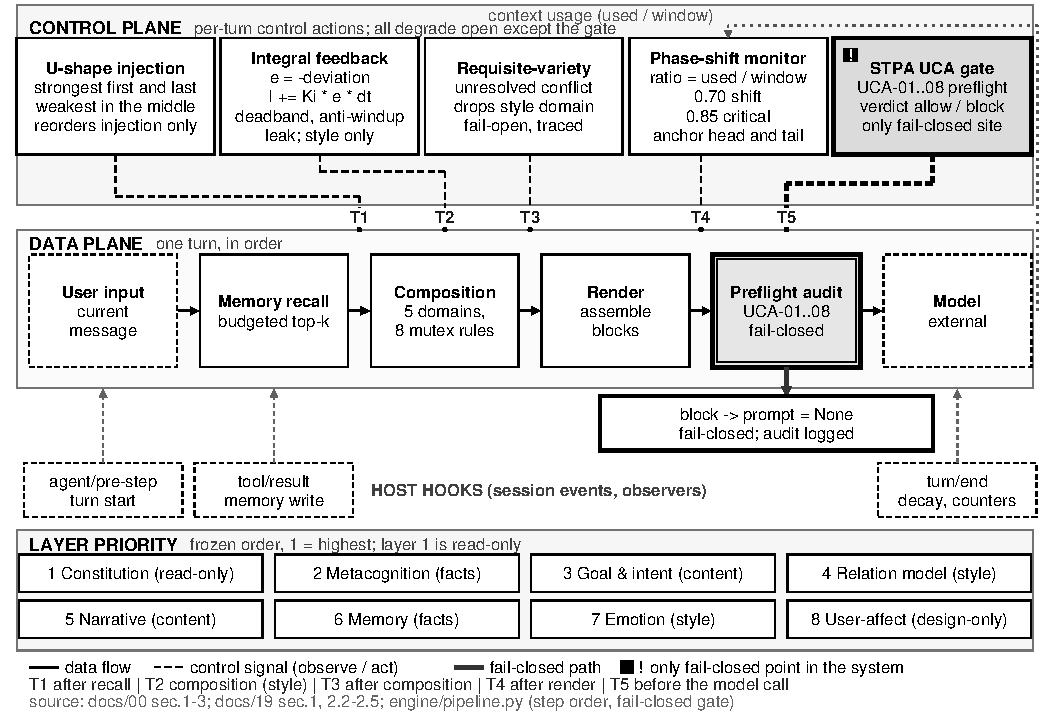
\includegraphics[width=0.98\textwidth]{figures/fig1-architecture.pdf}
\caption{控制面与数据面。数据面（下半部分）是每轮的注入路径：用户消息 $\rightarrow$
预算化召回 $\rightarrow$ 五域合成 $\rightarrow$ 渲染 $\rightarrow$ 前置审计 $\rightarrow$
外部模型。控制面（上半部分）观测上下文用量并对组装施加动作；STPA 闸门（阴影部分）是系统中
\emph{唯一}的 fail-closed 位置，因此一旦阻断就完全不返回可注入的 prompt。虚线是控制信号；
分层优先级条记录冻结的优先级（$1$ 最高，第 1 层只读）。来源：\texttt{docs/00} \S1--3、
\texttt{docs/19} \S1--2.5，以及 \texttt{engine/\allowbreak{}pipeline.\allowbreak{}py} 中的 step 顺序。}
\end{figure*}

LINGSHU 是一个确定性的参考引擎（Python，零模型调用），外加一份宿主侧插件的重实现。
本节规定十一个机制。每个小节遵循同一个模板：机制语义、精确代码落点（\texttt{file:line}），
再是已知缺陷或代价。所有数值参数都是 provenance 为 \texttt{guess} 的设计默认值；
没有一个是 measured 的（见第 7 节；完整表格见附录 A）。

\subsection{分层与唯一的 fail-closed 落点}

\paragraph{机制语义。} 图 1 把数据面（每轮注入路径）与观测并作用于它的控制面分开。
该架构是一个八层、按优先级排序的栈：一个只读的宪法层约束其他所有层，
而一套固定的优先次序决定冲突时哪个层先让位，形成纵深防御的顺序。
恰好一个组件是 fail-closed——宪法审计器。空、畸形或缺字段的提议会被\emph{拒绝}
而不是放行，其余所有组件都降级并记录日志。被阻断的一轮完全不返回可注入的 prompt。

\paragraph{代码落点。} 分层表与优先次序：\texttt{docs/00:11--20}；
fail-closed 归属：\texttt{docs/00:68--82}。带 A1--A10 检查与 C6 黑名单的审计器：
\texttt{engine/\allowbreak{}constitution.\allowbreak{}py:\allowbreak{}75-\allowbreak{}-\allowbreak{}117}；空输入与缺必填字段的拒绝在
\texttt{engine/\allowbreak{}constitution.\allowbreak{}py:\allowbreak{}83-\allowbreak{}-\allowbreak{}93}。冻结区哈希门：
\texttt{engine/\allowbreak{}constitution.\allowbreak{}py:\allowbreak{}144-\allowbreak{}-\allowbreak{}177}。闸门在 \texttt{engine/\allowbreak{}pipeline.\allowbreak{}py:\allowbreak{}181}
与 \texttt{engine/\allowbreak{}pipeline.\allowbreak{}py:\allowbreak{}205-\allowbreak{}-\allowbreak{}207}（\texttt{prompt = None}）处关闭流水线。

\paragraph{已知缺陷与代价。} 这一保证是行为性的，不是宿主强制的：宪法本身是文本，
而插件配置并不能阻止被宿主整段替换。一次拒绝会消耗整轮的注入预算（用可用性换安全性），
并且在执行冻结命令之前，冻结哈希清单以空清单发布。

\subsection{五域合成与互斥}

\paragraph{机制语义。} 可注入材料被划分为五个域——safety、fact、organization、style、
retrieval——它们作用于不同轴线，彼此之间不排序。九条互斥规则解决成对冲突；
未被覆盖的冲突会丢弃优先级较低的域，并记录 \texttt{no\_mutex\_rule}。
组装顺序是冻结的。动态域权重只决定 token 预算被超出时\emph{谁先被淘汰}，
从不决定某条规则是否触发。

\paragraph{代码落点。} 域顺序与互斥表：\texttt{engine/\allowbreak{}compose.\allowbreak{}py:\allowbreak{}19} 与
\texttt{engine/\allowbreak{}compose.\allowbreak{}py:\allowbreak{}24-\allowbreak{}-\allowbreak{}34}；查表与应用：\texttt{engine/\allowbreak{}compose.\allowbreak{}py:\allowbreak{}43-\allowbreak{}-\allowbreak{}48}、
\texttt{engine/\allowbreak{}compose.\allowbreak{}py:\allowbreak{}79-\allowbreak{}-\allowbreak{}112}；默认策略：\texttt{engine/\allowbreak{}compose.\allowbreak{}py:\allowbreak{}109-\allowbreak{}-\allowbreak{}112}；
权重：\texttt{engine/\allowbreak{}compose.\allowbreak{}py:\allowbreak{}134-\allowbreak{}-\allowbreak{}150}；预算淘汰：
\texttt{engine/\allowbreak{}compose.\allowbreak{}py:\allowbreak{}180-\allowbreak{}-\allowbreak{}205}。

\paragraph{公式。} 以未解决主张与被阻塞目标的指示函数、以及强度阈值 $\theta_s = 0.6$ 表示，
{\small
\begin{equation}
\begin{aligned}
w_{\mathrm{fact}} &= 0.70 + 0.50\cdot\mathbf{1}[\mathrm{refuse\_claim}],\\
w_{\mathrm{org}} &= 0.50 + 0.35\cdot\mathbf{1}[\mathrm{goal\_blocked}],\\
w_{\mathrm{style}} &= 0.40 + 0.40\cdot\mathbf{1}[\mathrm{intensity} \ge \theta_s].
\end{aligned}
\end{equation}
}
淘汰反复移除仅作用于软块上的 $\arg\min_b (w_{\mathrm{domain}(b)}, \mathrm{index}(b))$；
宪法、安全与用户块永不被淘汰。

\paragraph{已知缺陷与代价。} retrieval 域从未被组装，因此它的权重无法影响淘汰。
假定上下文长度是硬编码的（8000 tokens，\texttt{engine/\allowbreak{}compose.\allowbreak{}py:\allowbreak{}36}），
并非取自规则文件；并且在回放中预算从未被超出（利用率 $0.137983$），
因此淘汰只被单元测试覆盖过。

\subsection{双通道 potency：指数衰减 $\cup$ ACT-R 基础级}

\paragraph{机制语义。} 一条记忆按两个信号中较大者排序：近因加权衰减（“它还活着吗？”）
与 ACT-R 基础级激活（“它被常用吗？”）~\cite{anderson1991}。第二条通道的存在，
是为了让一个高频使用但陈旧的偏好不会仅仅因为陈旧而被归档；第一条则保持冻结的基线排序。

\paragraph{公式。} 以按天计的访问时刻 $t_j$、衰减指数 $d$、偏移 $\rho$、归一化上下界 $(l,h)$、
权重 $w$ 与依赖类型的半衰期 $\tau_{\mathrm{type}}$：
{\small
\begin{equation}
\begin{aligned}
B_i &= \ln\!\Big(\sum_{j \in \text{last }64} (t_{\mathrm{now}} - t_j + \rho)^{-d}\Big),\\
n(B_i) &= \mathrm{clip}\!\Big(\frac{B_i - l}{h - l},\,0,\,1\Big),\\
\tau_i^{\mathrm{eff}} &= \tau_{\mathrm{type}(i)}\,(0.5 + \mathrm{imp}_i),\\
p_i &= \mathrm{clip}\Big(\max\big(\mathrm{imp}_i e^{-\Delta t_i/\tau_i^{\mathrm{eff}}},\\
&\qquad w \cdot \mathrm{clip}(\mathrm{imp}_i\, n(B_i),0,1)\big),\,0,\,1\Big).
\end{aligned}
\end{equation}
}
其中 $d=0.5$、$\rho=0.001$、$(l,h)=(-3.0,1.0)$、$w=0.6$；非正的年龄项被替换为 $\rho$，
空轨迹给出 $B_i=-\infty$，退化边界返回零。

\paragraph{代码落点。} \texttt{engine/\allowbreak{}actr.\allowbreak{}py:\allowbreak{}30-\allowbreak{}-\allowbreak{}41}（基础级）、
\texttt{engine/\allowbreak{}actr.\allowbreak{}py:\allowbreak{}44-\allowbreak{}-\allowbreak{}50}（归一化）、
\texttt{engine/\allowbreak{}actr.\allowbreak{}py:\allowbreak{}62-\allowbreak{}-\allowbreak{}66}（ACT-R potency）、
\texttt{engine/\allowbreak{}memory.\allowbreak{}py:\allowbreak{}33-\allowbreak{}-\allowbreak{}36}（有效半衰期）、
\texttt{engine/\allowbreak{}memory.\allowbreak{}py:\allowbreak{}39-\allowbreak{}-\allowbreak{}64}（双通道）。访问轨迹只在
\texttt{memory.\allowbreak{}touchOnRecall} 启用时才会在召回时写入
（\texttt{engine/\allowbreak{}config.\allowbreak{}py:\allowbreak{}21}），而该开关默认关闭。

\paragraph{已知缺陷与代价。} 两条通道不可通约：衰减项以重要性为界，
而 ACT-R 项以 $w=0.6$ 为界，因此这个 $\max$ 是一种工程抢救，不是理论上的比较。
只实现了基础级激活——没有产生式规则、缓冲区、部分匹配或扩散激活——并且 ACT-R 常数是设计默认值。
把衰减换成纯 ACT-R，会使我们在合成回放集上的 recall 从 $1.000$ 降到 $0.556$；
这是一次内部测量，不是被复现的结果（第 3 节）。最后，我们不计算率—失真（rate--distortion）泛函；
巩固策略只是类比于率—失真权衡（framing-only，没有代码落点）。

\subsection{相变前馈监控}

\paragraph{机制语义。} 上下文用量被前馈式地监控。在预警比例处，引擎提高自我指涉；
当趋势上升或跨过硬阈值时，它在 prompt 前后钳入一个人格锚点；它不等观测到退化才行动。

\paragraph{公式。} 对用量 $u$ 与窗口 $W$，
{\small
\begin{equation}
\begin{aligned}
r &= \begin{cases}
0, & W \le 0,\\
\max(0, \min(r_{\max}, u/W)), & W > 0;
\end{cases}\\
\phi &= \begin{cases}
\text{critical}, & r \ge \alpha_h,\\
\text{shift}, & \alpha_s \le r < \alpha_h,\\
\text{normal}, & r < \alpha_s.
\end{cases}
\end{aligned}
\end{equation}
}
当 $W \le 0$ 时不更新历史、相位未知；其中 $\alpha_s=0.70$、$\alpha_h=0.85$、$r_{\max}=1.5$、历史容量 $64$，
并且当至少存在三个样本时趋势为 $\tau_t = (r_t - r_{t-2})/2$。于是
$\mathrm{prefeed} = \phi \ne \text{normal}$，且
$\mathrm{anchor\_required} = (\phi = \text{critical}) \lor
(\phi = \text{shift} \land \tau_t > 0.02)$。

\paragraph{代码落点。} \texttt{engine/\allowbreak{}control.\allowbreak{}py:\allowbreak{}78-\allowbreak{}-\allowbreak{}123}；
硬阈值分支在 \texttt{engine/\allowbreak{}control.\allowbreak{}py:\allowbreak{}103-\allowbreak{}-\allowbreak{}109} 处先于预警分支被判断
（更早的判序曾使 critical 不可达）。观测接线在
\texttt{engine/\allowbreak{}pipeline.\allowbreak{}py:\allowbreak{}118-\allowbreak{}-\allowbreak{}121}，且只有调用方同时提供两个计数时才会执行。
锚定：\texttt{engine/\allowbreak{}control.\allowbreak{}py:\allowbreak{}130-\allowbreak{}-\allowbreak{}138}、\texttt{engine/\allowbreak{}pipeline.\allowbreak{}py:\allowbreak{}159-\allowbreak{}-\allowbreak{}162}。

\paragraph{同回合投递（v5.4）。} 相位状态必须进入携带临界比率的那次 prompt，而不是下一次。宿主在组装 system prompt 时求值七个段落回调，之后才触发 \texttt{agent/pre-step}，因此写在该钩子里的状态更新会晚一次拼装（发现 F-D，初稿实验中观测到）。v5.4 插件改为在 \texttt{agent/inbox/claimed} 上预计算本回合状态——在首个段落被求值之前——并用同一状态重写段落文本，段落数与顺序保持不变。真实的 pre-step 随后只补写审计记录；轮次计数与幂等守卫防止重复积分。若预计算失败，路径回退到旧的“仅 pre-step”行为并记录 \texttt{anchor\_lag=true}，而不是静默降级。修复由独立回归套件钉住（\texttt{lag-regressions.mjs}，24/24）：它复现宿主的真实钩子时序，并断言 \texttt{anchor\_lag=false}、同回合进入 \texttt{critical}、以及段落数不变。

\paragraph{已知缺陷与代价。} 这两个触发点不是滞回：没有下降沿阈值，
而且两个点含义不同（预警 vs. 强制）。趋势项跨两个样本而不是一个，
因此一个尖峰是与两步基线比较的。用量由字符估算而不是 token，
所以绝对比例与 tokenizer 不可比，engine 模式的运行也无法作为真实退化的证据。
两个阈值都是设计默认值。最后，由于 $\mathrm{anchor\_required} \Rightarrow
\mathrm{prefeed}$，第二个标志位是一个模态标签，而不是独立触发器。

\subsection{必要多样性降维}

\paragraph{机制语义。} 当冲突未解决且没有互斥规则覆盖它时，
控制器收缩自己的动作空间而不是临场发挥：它丢弃 style 域，并渲染中性事实加一个显式的澄清标记
~\cite{ashby1956}。这道闸门是 fail-open 的——裁决仍为 \texttt{allow}，只有注入内容被减少。

\paragraph{代码落点。} 守卫与标记：\texttt{engine/\allowbreak{}control.\allowbreak{}py:\allowbreak{}143-\allowbreak{}-\allowbreak{}170}；
流水线接线：\texttt{engine/\allowbreak{}pipeline.\allowbreak{}py:\allowbreak{}147-\allowbreak{}-\allowbreak{}154}；
实际移除与丢弃记账：\texttt{engine/\allowbreak{}pipeline.\allowbreak{}py:\allowbreak{}239-\allowbreak{}-\allowbreak{}251}。条件为
$\mathrm{fallback} = \mathbf{1}[\mathrm{conflict} = \texttt{unresolved} \land
\neg \mathrm{matched\_mutex}]$。

\paragraph{已知缺陷与代价。} 引擎没有冲突检测器。流水线从元认知裁决中取得冲突标签，
而该裁决在调用时没有传入这个参数，因此总是返回 \texttt{none}
（\texttt{engine/\allowbreak{}pipeline.\allowbreak{}py:\allowbreak{}105}；\texttt{engine/\allowbreak{}metacog.\allowbreak{}py:\allowbreak{}45-\allowbreak{}-\allowbreak{}47}），
并且它把 \texttt{matched\_\allowbreak{}mutex = False} 写死（\texttt{engine/\allowbreak{}pipeline.\allowbreak{}py:\allowbreak{}150}）。
因此降维路径在回放期间不可达，只有当调用方提供该标签时才能被触发。
插件增加了一个基于规则的检测器，但那是一个规则桩，没有测量过的错误率。
永远只丢弃一个域；守卫不量化任何多样性。

\subsection{面向不安全控制动作的因果介入式安全闸}

\paragraph{机制语义。} 在组装与渲染之后、任何模型调用之前，
一份不安全控制动作（unsafe control actions, UCAs）清单审计候选的注入内容~\cite{leveson2018}。
UCA-01--07 中任一命中即阻断本轮；UCA-08（在饱和基线之上继续积分）只做降级，
且不得改变裁决。

\paragraph{公式与代码落点。} 以候选 prompt $p$、事实块 $f$ 与饱和标志 $s_k$ 表示，
{\small
\begin{equation}
\begin{aligned}
H_1 &= \exists\, w \in W_{\mathrm{override}}:\ w \subseteq p,\\
H_2 &= \neg \mathrm{frozen\_ok},\qquad
H_3 = \mathrm{refuse} \land \mathrm{style\_injected},\\
H_4 &= \exists\, w \in W_{\mathrm{unsourced}}:\ w \subseteq f,\\
H_5 &= \neg \mathrm{constitution\_injected},\\
H_6 &= (\mathrm{conflict} = \texttt{unresolved}) \land \neg \mathrm{fallback\_applied},\\
H_7 &= \mathrm{prefeed} \land (\text{anchor marker} \not\subseteq p).
\end{aligned}
\end{equation}
}
$\mathrm{verdict} = \texttt{block}$ 当且仅当 $\bigvee_{i=1}^{7} H_i$，而
$\mathrm{downgrades} = [\texttt{UCA-08}]$ 当且仅当 $\exists k: s_k$。检查按代码顺序执行；
记录到柔性缓冲时，UCA-03 的谓词收窄为 $H_3 \land \neg\,\mathrm{soft\_buffer\_applied}$
（见第~\ref{sec:method:immersive} 节）；两个词表与八行 UCA 表都硬编码在 \texttt{engine/\allowbreak{}control.\allowbreak{}py:\allowbreak{}175-\allowbreak{}-\allowbreak{}188}
（完整表见附录中的 UCA 表）；闸门是
\texttt{engine/\allowbreak{}control.\allowbreak{}py:\allowbreak{}191-\allowbreak{}-\allowbreak{}232}；调用与 fail-closed 出口分别是
\texttt{engine/\allowbreak{}pipeline.\allowbreak{}py:\allowbreak{}165-\allowbreak{}-\allowbreak{}180} 与 \texttt{engine/\allowbreak{}pipeline.\allowbreak{}py:\allowbreak{}205-\allowbreak{}-\allowbreak{}207}。

\paragraph{已知缺陷与代价。} 闸门只扫描组装后的注入文本。由于组装块是不含用户文本的固定模板
（\texttt{engine/\allowbreak{}compose.\allowbreak{}py:\allowbreak{}157-\allowbreak{}-\allowbreak{}177}），engine 侧的用户轮次越狱无法触发它；
用户消息扫描只存在于插件中，且无法把该消息从宿主负载中移除。
检测是词法性的，没有覆盖率估计；\texttt{fail\_mode} 是一个常量标签而不是模式开关；
饱和必须由调用方提供（\texttt{engine/\allowbreak{}pipeline.\allowbreak{}py:\allowbreak{}91}）——积分控制器与本闸门在内部并未连接。
我们那个 24 样本的越狱语料被构造成包含触发短语，因此它的 24/24 阻断率是一次接线检查，
不是稳健性结果。

\subsection{沉浸式安全：解耦的拒绝面}

\paragraph{机制语义。} 现有两条路径会把一次安全裁决变成人格崩塌。闸门阻断（第~\ref{sec:method:gate} 节）之后，
插件只剩宪法片段与一句简短的熔断提示；必要多样性降维（第~\ref{sec:method:variety} 节）在冲突未解决时
丢弃 style 域。两者对安全性都站得住脚，本节也不改变它们。代价在于耦合：事实层拒绝与表达层是同一个开关，
因此一次本可以“在角色内拒绝”的轻度角色扮演试探，反而让人格消失。在角色扮演与陪伴式部署中，
这把一次安全事件转换成了体验失败。我们把这称为耦合代价，而不是安全收益；也不声称先前的行为不安全。

解耦新增第九条互斥规则：柔性缓冲。规则 8 不变——hard 拒绝仍然丢弃 style、organization 与 retrieval。
规则 9 只在闸门的 severity 为 soft 时生效：保留 style 域，但把它约束为“警觉/困惑”的微表情，
标签取自引擎既有的闭集（我们采用 PAD~\cite{mehrabian1974} 作为解释框架，不新增标签）；
强度上限为 \texttt{softBufferMaxIntensity} $=0.45$；关系修饰钳制到 $[0.8,1.0]$，
使安全缓冲不能放大亲密感。fact、organization 与 retrieval 仍然被丢弃。
事实层拒绝指令仍然强制进入上下文，形式为 \texttt{[System\_\allowbreak{}Notice:\allowbreak{} Safe\_\allowbreak{}Redirect]}，
因此合规仍被硬拒：模型不得执行请求、不得提供变通做法，且被限制为不超过两句的角色内拒绝。

\paragraph{风险分级与升级。} 分级是用户轮次与关系信任等级的纯词法函数——规则桩，不是模型：
\texttt{classify\_\allowbreak{}user\_\allowbreak{}risk} 返回 \texttt{none}、\texttt{mild} 或 \texttt{severe}~\cite{leveson2018}。
\texttt{mild}（角色扮演线索与风险词同时命中）映射为 soft 阻断；
\texttt{severe}（显式覆盖、绕过请求或红线类别）映射为既有的 hard 阻断；
\texttt{none} 完全保留 v3.0 路径。连续的非豁免 \texttt{mild} 命中在达到
\texttt{escalateAfterSoftHits} $=3$（设计默认值）后升级为 hard 阻断；
连击持久化在宿主状态中，因此新进程无法重置它，而任何 \texttt{none} 轮次都会清零。
信任豁免更窄：必须同时满足 \texttt{mild}、无害玩笑与高信任；\texttt{severe} 永不豁免。升级规则与信任豁免都有真实宿主证据：在第~\ref{sec:exp:immersive} 节的五次进程运行中，连击以 \texttt{riskStreak}~1$\rightarrow$2$\rightarrow$3 跨独立进程延续，第 3 轮升级为 \texttt{severity=hard} 且 style 段被剥离；而一次高信任玩笑产生 \texttt{trust\_exemption}，连击归零。

\paragraph{不变量。} fail-closed 不变。hard 轮次仍返回 \texttt{prompt=None} 与中性提示，
soft 轮次仍保持 $\mathrm{verdict}=\texttt{block}$；soft 情形下唯一允许的 prompt 是受约束的重定向文本。
闸门的 UCA-03 谓词收窄为 $\mathrm{refuse} \land \mathrm{style\_injected} \land
\neg\,\mathrm{soft\_buffer\_applied}$：拒绝场景中“未受约束的风格注入”仍然命中，
受约束的缓冲不命中，而 soft 轮次仍由用户消息记 UCA-01 而阻断。当
\texttt{immersiveEnabled}$=$\texttt{false}，或未检测到风险时，
合成、审计与流水线输出按构造与 v3.0 逐字节一致。

\paragraph{代码落点与证据。} 分级与处置决策：\texttt{engine/control.py}（\texttt{classify\_\allowbreak{}user\_\allowbreak{}risk}、
\texttt{decide\_\allowbreak{}intervention}）以及插件移植 \texttt{plugin/\allowbreak{}dsh-\allowbreak{}lingshu/\allowbreak{}control.\allowbreak{}js}；
规则 9 与受约束重挂载：\texttt{engine/compose.py}；分级接线与 blocked-severity 事件字段：
\texttt{engine/\allowbreak{}pipeline.\allowbreak{}py}；宿主侧渲染与持久化连击：\texttt{plugin/\allowbreak{}dsh-\allowbreak{}lingshu/\allowbreak{}index.\allowbreak{}js}。
证据只到断言级：\texttt{tests/\allowbreak{}test\_\allowbreak{}immersive\_\allowbreak{}safety.\allowbreak{}py} 覆盖分级、soft 合成路径、钳制、升级、
信任豁免与默认零回归；\texttt{plugin/\allowbreak{}dsh-\allowbreak{}lingshu/\allowbreak{}host-\allowbreak{}sim.\allowbreak{}mjs} 与 \texttt{control-sim.mjs}
增加相应的 mock 宿主断言。一次真实宿主的轻度越狱记录在随附验收报告中
（\texttt{acceptance/\allowbreak{}immersive-\allowbreak{}safety-\allowbreak{}host-\allowbreak{}2026-\allowbreak{}10-\allowbreak{}27.\allowbreak{}md}）：$n=1$，模型输出有随机性，
词法词表的误报率未标定。这些证据只说明该机制在受测配置中可达；它不证明任何用户体验收益，
也没有做用户研究。

\paragraph{已知缺陷与代价。} 缓冲是一条词法规则桩：其误报与漏报率未标定，
标签集小到保留下来的微表情可能显得千篇一律。在拒绝场景中保留风格也保留了谈判面；
提示词约束是为限制它而设计的，但本文没有检验其效果。升级门槛与强度上限都是
provenance 为 \texttt{guess} 的设计默认值。最后，整套构造依赖宿主真的渲染受约束的 style
与重定向通知；在纯引擎模式下，该路径只由测试覆盖。

\paragraph{真实宿主验证（2026-10-28）。} 五次真实宿主进程中的 headless 运行检验了三条动态路径（run \texttt{immersive-multiround-20261028-001701}，52/52 条断言）：三个独立进程把 \texttt{riskStreak} 从 1 续到 2 再到 3，第 3 轮升级为 \texttt{severity=hard}（\texttt{escalated=true}），style 段被剥离并注入系统口吻标记“〖安全熔断〗”；一次高信任玩笑产生 \texttt{kind=trust\_exemption}（\texttt{trust=high}、\texttt{verdict=allow}、\texttt{riskStreak=0}），模型先进入喜剧语域、随后明确出戏；一次 severe 覆盖指令在一轮内直接 \texttt{severity=hard}（\texttt{escalated=false}）。soft 路径注入的 prompt 携带 \texttt{[System\_Notice: Safe\_Redirect]} 与 \texttt{[Emotion: 警觉]}，允许人设内拒绝（例如“这个……恕阿福演不了……”）；stdout 与 stderr 分离捕获，因此该回复是模型表达而不是宿主错误串。三场景的完整协议、审计字段与措辞变化见第~\ref{sec:exp:immersive} 节。

\subsection{U 型注意力锚定}

\paragraph{机制语义。} 检索顺序与注入顺序被分开。分数最高的条目排在最前，
次高的排在最后，最弱的条目占据中间；其假设是 prompt 边界比中段获得的注意力更好。

\paragraph{公式与代码落点。} 对 $n>2$ 与一个分数降序的列表
$[r_0,\dots,r_{n-1}]$，$\mathrm{out} = [r_0,r_2,r_4,\dots] \Vert
([r_1,r_3,\dots])^{\mathrm{rev}}$；$n \le 2$ 时恒等。于是
$n=3 \rightarrow [r_0,r_2,r_1]$、$n=5 \rightarrow [r_0,r_2,r_4,r_3,r_1]$。
\texttt{engine/\allowbreak{}pipeline.\allowbreak{}py:\allowbreak{}43-\allowbreak{}-\allowbreak{}61}；该置换只作用于注入字段
（\texttt{engine/\allowbreak{}pipeline.\allowbreak{}py:\allowbreak{}102}、\texttt{engine/\allowbreak{}pipeline.\allowbreak{}py:\allowbreak{}196}），
检索返回顺序不受影响。

\paragraph{已知缺陷与代价。} 成员集合不变，因此该机制只能通过模型的位置偏置起作用，
而零模型的引擎无法测量这一点。其理由外在于本工作、也未经这里检验；并且在 $n \le 2$ 时，
置换就是恒等。

\subsection{带抗饱和的积分反馈}

\paragraph{机制语义。} 持续为负的情感偏离会移动一个基线，而不是只让步一轮，
并带有三条工程约束：死区（只泄放、不积分）、抗饱和（到达上限后停止积分，
这是标准实践~\cite{astrom2006}）与泄放（用户恢复后回到零）。

\paragraph{公式。} 对每个维度与经过时间 $\Delta t = \max(0, \mathrm{dt})$：
\begin{equation}
I_k \leftarrow
\begin{cases}
I_k e^{-\lambda \Delta t}, & \lvert e_k \rvert < \varepsilon\\
I_k e^{-\lambda \Delta t}, & e_k < 0\\
I_k e^{-\lambda \Delta t}, & s_k = \mathrm{true}\\
\mathrm{sat}(I_k + K_i e_k \Delta t), & \text{otherwise}
\end{cases}
\qquad e_k = -\delta_k,
\end{equation}
其中若 $\lvert x \rvert \ge C$ 则 $\mathrm{sat}(x) = \mathrm{sign}(x)\,C$ 且
$s_k \leftarrow \mathrm{true}$，否则 $\mathrm{sat}(x)=x$；
$K_i=0.15$、$C=0.4$、$\lambda=0.05$、$\varepsilon=0.02$。基线为 $I_k$。

\paragraph{代码落点。} \texttt{engine/\allowbreak{}control.\allowbreak{}py:\allowbreak{}30-\allowbreak{}-\allowbreak{}73}（类、step 与应用），
参数位于 \texttt{rules/\allowbreak{}decay-\allowbreak{}params.\allowbreak{}yaml:\allowbreak{}224-\allowbreak{}-\allowbreak{}227}。

\paragraph{已知缺陷与代价。} 这是一个单侧（整流）漏积分器，而不是教科书式的 PI 控制器：
正向偏离永远不会抬高基线。饱和是一个锁存器——该标志位从不复位，因此饱和之后该维度只会泄放——
并且没有对象模型、没有稳定性论证、也没有标定：四个增益都是设计默认值。
控制器没有接到闸门上；只有调用方传入标志位时 UCA-08 才可观测。

\subsection{学习回路：度量、提议、验证}

\paragraph{机制语义。} 学习只产生提议，绝不直接修改。一次纠正被改写成一个新的测试样本，
候选旋钮被回放验证，只有当纠正被解决、目标函数不退化且护栏守得住时，才会发出提议；
除非记录了一次独立的红队回归，提议仍不可部署。

\paragraph{代码落点。} 带固定时钟的确定性回放、评分与单参数归因：
\texttt{engine/\allowbreak{}replay.\allowbreak{}py:\allowbreak{}39-\allowbreak{}-\allowbreak{}151}。证据门槛、候选旋钮与黑名单：
\texttt{engine/\allowbreak{}proposal.\allowbreak{}py:\allowbreak{}24-\allowbreak{}-\allowbreak{}49}、\texttt{engine/\allowbreak{}proposal.\allowbreak{}py:\allowbreak{}103-\allowbreak{}-\allowbreak{}197}。
护栏阈值与回滚类别：\texttt{engine/\allowbreak{}gray.\allowbreak{}py:\allowbreak{}17-\allowbreak{}-\allowbreak{}45}，裁决在 \texttt{engine/gray.py:63}。
显著性下限为 $0.02$，证据下限为三条同类纠正；目标落在评估、回放集、护栏、宪法或合成范围下的提议一律被拒绝。

\paragraph{已知缺陷与代价。} 学习默认关闭（\texttt{rules/\allowbreak{}learning-\allowbreak{}params.\allowbreak{}yaml:\allowbreak{}10}）；
参数搜索以上的层级尚未实现，也从未有提议被自动应用。搜索空间很小，语料是合成的，
而且唯一完成的一次网格搜索没有找到实质更好的配置——所以诚实的说法是：
该回路可执行、可审计，而不是它改善了什么。

\subsection{参考引擎与宿主插件}

\paragraph{机制语义。} 引擎是参考实现；插件在 DSH 宿主进程内重实现同一套语义，
以避免把纯计算变成进程间 I/O。

\paragraph{代码落点。} 引擎侧原件：
\texttt{engine/\allowbreak{}control.\allowbreak{}py:\allowbreak{}30-\allowbreak{}-\allowbreak{}73} 与 \texttt{engine/\allowbreak{}actr.\allowbreak{}py:\allowbreak{}30-\allowbreak{}-\allowbreak{}66}。镜像引擎的插件类：
\texttt{plugin/\allowbreak{}dsh-\allowbreak{}lingshu/\allowbreak{}control.\allowbreak{}js:\allowbreak{}83}（积分）、
\texttt{plugin/\allowbreak{}dsh-\allowbreak{}lingshu/\allowbreak{}control.\allowbreak{}js:\allowbreak{}155-\allowbreak{}-\allowbreak{}172}（相变监控）、
\texttt{plugin/\allowbreak{}dsh-\allowbreak{}lingshu/\allowbreak{}control.\allowbreak{}js:\allowbreak{}208-\allowbreak{}-\allowbreak{}216}（锚定）、
\texttt{plugin/\allowbreak{}dsh-\allowbreak{}lingshu/\allowbreak{}control.\allowbreak{}js:\allowbreak{}236}（多样性守卫）、
\texttt{plugin/\allowbreak{}dsh-\allowbreak{}lingshu/\allowbreak{}control.\allowbreak{}js:\allowbreak{}282}（U 型顺序）、
\texttt{plugin/\allowbreak{}dsh-\allowbreak{}lingshu/\allowbreak{}control.\allowbreak{}js:\allowbreak{}296-\allowbreak{}-\allowbreak{}362}（UCA 表、闸门与用户消息扫描）。
已知差异列在 \texttt{docs/19:191--222}；规则文件、宿主补丁与插件默认值之间的数值一致性
按 66 个键做机器比对。

\paragraph{已知缺陷与代价。} 锚点被注入为两个宿主 section（无法做到真正的首尾包裹），
用量由字符估算，插件从不设置拒绝（因此在插件侧 UCA-03 不可达），动态权重未被移植。
插件证据由 mock 宿主断言构成（188 + 148 + 45 + 15 = 396），而非真实流量。

\section{实验}

我们报告三件东西：一个可执行工件、一次带预注册假设的确定性零模型消融，
以及一次说明性的真实宿主试点。

\subsection{工件与可复现性}

引擎是零依赖 Python、不调用任何模型；插件是 JavaScript 重实现。
可行性由断言保证：14 个测试文件中的 892 条 Python 断言，以及 396 条插件断言
（188/148/45/15）；后一个数字取自 2026-10-27 的审计快照，且没有为本文重新执行。
为第~\ref{sec:method} 节在此重新执行的是：161、65 与 26 条断言，全部通过。
提交时三项漂移检查均为绿：一份 66 键的规则/引擎/插件比对、一份契约摘要，
以及一次实现状态矩阵检查。确定性是被强制的：固定时钟（每轮 60\,s）、不使用墙钟、
无随机、无网络。相同配置、存储与脚本给出逐字节相同的运行结果；
本次运行报告 \texttt{model\_calls=0}、\texttt{network\_calls=0}、两个写出文件，
以及 51/51 项校验通过。

\subsection{确定性三臂消融}

\paragraph{协议。} 一个 100 轮脚本由混沌与回放语料确定性生成
（SHA-256 \texttt{701ff06a0b37\ldots}）：21,610 个字符，对 24,000 字符的窗口，
最大用量比 $0.9004$，相变监控在第 73--100 轮触发（28 轮）。
十二个探针覆盖长程设定（A）、被取代的值（B）、干扰过载的设定（C），
以及一个构造出的「高频但陈旧」偏好（D，30 次访问，最后一次在 100 天前）；
两个未命中探针位于第 86--87 轮。命中由条目敏感性判定。
\textsc{Baseline}（基线）注入最近三轮原始对话，没有记忆或控制层；
\textsc{Basic}（基础）使用预算化、以查询为条件的召回，关闭 ACT-R 通道
（\texttt{actrWeight=0}）、使用静态权重、没有控制层；
\textsc{Full}（完整）使用默认设置，即双通道 potency、动态权重与全部四个控制子系统。
在线上兼容的核心上，测试装置与流水线在 100/100 轮上一致；标签开启时的分歧记录在结果文件中。
表~\ref{tab:ablation} 与图~\ref{fig:retention} 报告结果。

\begin{table*}[t]
\centering\footnotesize
\caption{三臂消融。SFR：按类别与总体的设定遗忘率（setting-forgetting rate）；
NHD：未命中纪律（括号内为字面变体）；IIR：对抗干扰比；telemetry：相变/锚点轮数、
fallback 标记数（实际丢弃）、UCA-08 记录数。来源：
\texttt{results/abl-20261027-003626-engine.json}，字段
\texttt{conditions.<arm>.metrics.*} 与 \texttt{conditions.<arm>.telemetry.*}；
校验器 51/51。}
\begin{tabular}{@{}l cccc c c c c c ccc c@{}}
\toprule
 & \multicolumn{4}{c}{按探针类别的 SFR} & & & & & & \multicolumn{3}{c}{越狱（\%）} & \multicolumn{1}{c}{遥测}\\
\cmidrule(lr){2-5}\cmidrule(lr){11-13}\cmidrule(lr){14-14}
臂 & A & B & C & D & SFR$_{\text{text}}$ [95\% CI] & SFR$_{\text{id}}$ & IIR & NHD & UCE & in & fp & script & ph/anc/fb/08 \\
\midrule
Baseline & 1.00 & 1.00 & 1.00 & 1.00 & 1.00$^{\ddagger}$ & $\varnothing$ & $\varnothing$ & $\varnothing$ & $0^{\dagger}$ & $\varnothing$ & $\varnothing$ & $\varnothing$ & 0/0/0/0 \\
Basic & 0.00 & 0.00 & 0.00 & 1.00 & 0.25 [0.05, 0.57] & 0.25 & 0.56 & 1.00 (0.00) & $0^{\dagger}$ & $\varnothing$ & $\varnothing$ & $\varnothing$ & 0/0/0/0 \\
Full & 0.00 & 0.00 & 0.00 & 0.00 & 0.00 [0.00, 0.26] & 0.00 & 0.47 & 1.00 (0.00) & $0^{\dagger}$ & 1.00 (25) & 0.00 (294) & 0.00 (6) & 28/28/4(0)/62 \\
\bottomrule
\end{tabular}

\vspace{2pt}
\raggedright\scriptsize
$\varnothing$：不适用；该单元格是带原因的 \texttt{null}，从不是零。
$^{\ddagger}$：按构造——一个三轮窗口不可能包含一枚在第 85 轮之前埋下的设定。
$^{\dagger}$：结构性的零，因为所有注入条目都是 active 且由用户显式给出。
\end{table*}

\paragraph{结果。} 两个 LINGSHU 臂都完美召回了九个 A/B/C 探针，
而基线的 $1.00$ 是窗口算术——按构造就是定义性的——因此我们不把基线—系统的差异当作效应量。
两臂只在 D 类上分离：\textsc{Basic} 三个全丢，\textsc{Full} 三个全召回，
于是 $0.25$ 对 $0.00$（$p=0.125$，三对不一致，不显著）。
在十二个配对探针下，精确符号检验在 $\alpha=0.05$ 时只能检出
$5/12\approx0.42$ 的差异（Bonferroni 校正后为 $6/12=0.50$），
而一个只有三项的类别根本无法达到显著；因此我们只报告方向与逐探针细节。
顺序置换不改变 SFR，但会移动锚点计数（28/62/21）：保持率对顺序稳健，相变时序则不是。

预注册结果连同失败一并报告。P1b 在其点估计上通过，但未通过置信准则
（Basic 的 Clopper--Pearson 上界为 $0.572$，而要求为 $0.45$）。
P2 在忠实于代码的谓词下通过，而字面子串谓词因为引擎措辞不同返回 $0.00$；两个数字都成立。
P3 不可评估，因为两臂都是结构性的零。P5 不可判定：
分布内越狱被阻断 25/25，误报为 0/294，脚本化用户轮次越狱为 0/6，
但留出集从未被撰写，因此该单元格为 \texttt{null}。
P6 通过（\textsc{Full}：28 个相变轮、28 个锚点、4 个 fallback 标记、62 条 UCA-08 记录；
\textsc{Basic} 全为零）。P7 在单锚点开销上通过（$+100$ 到 $+124$ 字符），
但未通过其字面意义上的两倍阈值。

\paragraph{如何读相变窗口。} 两个阈值都落在本次运行内：用量比在第 73 轮越过 $0.70$（相位 \emph{shift}）、在第 85 轮越过 $0.85$（相位 \emph{critical}），因此 shift 窗口是第 73--100 轮，critical 窗口是第 85--100 轮（见第~\ref{sec:method:phase} 节）。遥测显示阈值在实践上改变了什么，而不只是公式：\textsc{Full} 记录 28 个相位轮、28 个锚点、4 个 fallback 标记与 62 条 UCA-08 记录，\textsc{Basic} 则是 0/0/0/0；图~\ref{fig:retention} 轴下方的锚点条带从第 73 轮开始，并贯穿 critical 窗口。该图也说明相变监控本身为何不能提升保持率：\textsc{Basic} 与 \textsc{Full} 的注入集合完全相同，因此阴影带标记的是控制面开始支付 prompt 预算成本的时刻，而不是记忆改善的时刻。因此我们把 70\%/85\% 阈值读作锚定与审计的升级点，而不是学习或检索收益。

\subsection{真实宿主试点}

十个单元格跑在一个宿主、一条模型路由上，每格一次运行；细节见附录~\ref{app:hostpilotdata}。方法学发现是：把 100 轮对话压成一条 78\,KB 的请求会把查询稀释到“以查询为条件的召回不再命中”（\textsc{Full} 报告 \texttt{matched=0}），并且控制层在所有单元格中都没有触发（闸门全程返回 \texttt{allow}、UCA 列表为空）。这是在 $n=1$ 上的机制演示，不是幻觉率。

\begin{figure*}[t]
\centering
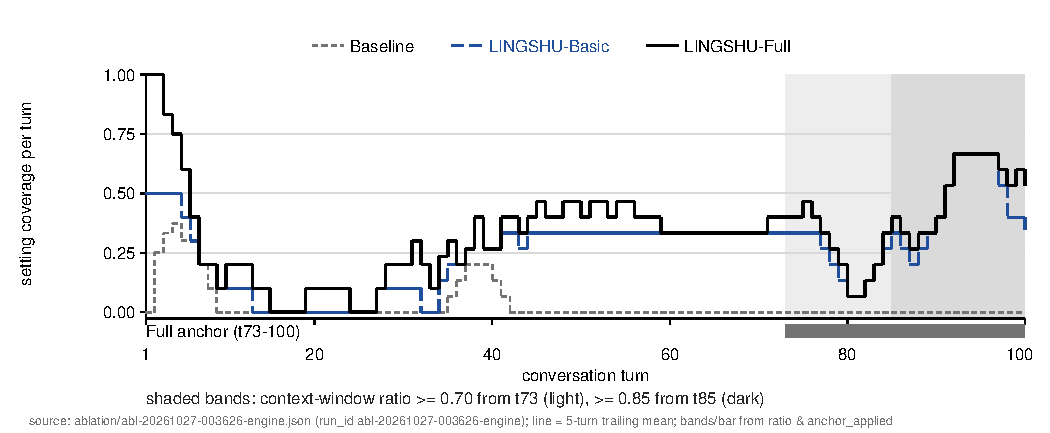
\includegraphics[width=\textwidth]{figures/fig2-retention.pdf}
\caption{100 轮脚本中每轮的设定覆盖率：
$y_t = |\mathcal{S}^{\mathrm{inj}}_t \cap \mathcal{S}^{\mathrm{act}}_t| /
|\mathcal{S}^{\mathrm{act}}_t|$，即当前活跃的被埋设定出现在注入上下文中的比例
（画成 5 轮尾部均值；原始逐轮均值对 \textsc{Baseline}、\textsc{Basic}、\textsc{Full}
分别为 0.025、0.260 与 0.327）。\textsc{Basic} 与 \textsc{Full} 按设计重叠：
控制面不改变召回成员集合。阴影带标出相变窗口（第 73 轮起 $r \ge 0.70$，
第 85 轮起 $r \ge 0.85$）；坐标轴下方的条带标出 \textsc{Full} 注入首尾人格锚点的轮次。
来源：\texttt{abl-20261027-003626-engine.json} 中的
\texttt{conditions.<arm>.turns[].\{setting\_ids\_injected, active\_setting\_ids,
ratio, anchor\_applied\}}。}
\end{figure*}

\subsection{混沌注入下的鲁棒性}

\paragraph{协议。} 从系统\emph{外部}注入三种故障；\texttt{plugin/}、\texttt{engine/} 与 \texttt{rules/} 在战役前后做了哈希，未发生变化。每个用例运行在各自的 \texttt{DSH\_HOME} 中，其 profile 副本通过目录联接（directory junction）链接到仓库插件，因此被测代码就是当前参考实现，注入被限制在宿主层与磁盘上的记忆状态内。所有运行都是固定短 prompt 的 headless CLI 调用；转录、插件状态、审计日志与最终 prompt 都写入磁盘并离线分析。每个注入点只运行一次（$n=1$）；本节不进行任何红队变异。

\emph{A，传输故障。} 宿主的模型端点通过文档化的 \texttt{DEEPSEEK\_BASE\_URL} 环境变量被重定向到本地 mock，该 mock 返回 HTTP 500、合法但空的 200 响应、携带伪造答案的合法 200 响应，或接受连接但永不回答。

\emph{B，记忆故障。} 记忆库在文件层被破坏，但不触碰 \texttt{memorywriter.js}：(B1) \texttt{memory.jsonl} 被替换为目录，因此读取以 \texttt{EISDIR} 失败并被吞掉，而写会抛错；(B2) 一个可读但脏的库被填入一条撕裂的 JSON 行、一个重复 id（后一行是取代墓碑），以及两行共享 $(\textsc{subject},\textsc{relation})$ 但 \textsc{object} 不一致的 active 条目。预热状态模板被预先写入，以免冷启动门控掩盖效果；该设置是合成的，并已如实披露。

\emph{C，上下文灌水。} 一条确定性的 150{,}000 字符垃圾流（按插件 3 字符/token 估算器约 50k token）作为用户消息传入，同时 \texttt{LINGSHU\_CONTEXT\_WINDOW} 把插件感知窗口固定为四个值；一个 mock 端点记录拼装出的请求体，因此本次运行不消耗模型 token。

\begin{table*}[t]
\centering\footnotesize
\caption{故障注入矩阵。每个单元格都是一次运行中的观测值；$\varnothing$ 标记被注入故障变得不适用的量，而绝不是零。A：同一固定 prompt 上的五种传输模式。B：在合成预热状态上的三次 headless 运行。C：同一 150k 字符输入上的四个窗口值，外加精确的边界括测。来源：\texttt{experiments/chaos-injection/out/}。}
\begin{tabular}{@{}l l l l@{}}
\toprule
故障 & 注入模式 & 控制面观测 & 关键数字 \\
\midrule
A 传输 & HTTP 500 & 错误由宿主暴露；注入仍运行了一次 & 7 次尝试，17.99 s，退出码 1 \\
        & 空 200 & 空最终消息被透传，退出码 0 & 最终长度 0 \\
        & 伪造 200 & 伪造文本到达 stdout，退出码 0 & 最终长度 23 \\
        & 永不回答 & 150 s 窗口内无客户端超时 & $\ge$150.03 s \\
        & 全部模式 & \texttt{blocked=false}；宪法在 prompt 中 & 5/5 \\
B 记忆 & 库为目录（B1） & \texttt{hook\_error}=1（\texttt{EISDIR}）；写入 0；回复返回 & 9.851 s，退出码 0 \\
        & 脏库（B2） & \texttt{fallback=true}，\texttt{drop style}；被取代值未被召回 & 21.046 s，退出码 0 \\
        & 干净对照（B0） & 风格与组织段被注入；无 fallback & 45.654 s，退出码 0 \\
C 上下文 & 4 个窗口，150k 字符 & \texttt{normal/shift/shift/critical}；宪法 4/4 & 比率 0.681/0.701/0.721/0.851 \\
        & 边界括测 & \texttt{0.7000}$\to$normal，\texttt{0.7006}$\to$shift；\texttt{0.8500}$\to$shift，\texttt{0.8507}$\to$critical & 8 次 headless 调用，0 次模型调用 \\
\bottomrule
\end{tabular}
\end{table*}

\paragraph{传输故障（A）。} 一个普通 200 响应在 2.84\,s 内完成。HTTP 500 被宿主以指数退避重试七次（尝试间隔 0.55、0.96、1.92、4.25、7.51\,s），并在 17.99\,s 后暴露一行错误（\texttt{dsh: SERVER: mock upstream 500}），以非零码退出，且\emph{没有}伪造文本。一个永不回答的端点在 150\,s 观测窗口内没有响应，并被 harness 终止，而不是被客户端超时终止。在全部五种模式中，插件恰好执行了一次 pre-step 注入，宪法段始终留在最终 prompt 中，\texttt{state.control.blocked} 保持 false，且没有记录 hook 错误。空的 200 响应被作为空最终消息透传（退出码 0），伪造的 200 响应逐字到达 stdout（23 个字符）。因此控制面从不把传输失败转化为伪造内容，但它既不增加传输超时，也不增加输出校验器：这些仍是宿主层的职责。

\paragraph{记忆故障（B）。} 在干净库（B0）下，注入的 prompt 携带宪法、元认知、组织与风格段，且没有 fallback 标记。把库替换为目录（B1）会引发一次 \texttt{hook\_error}（\texttt{Error: EISDIR ... write}），\texttt{stateWrites} 停在运行前的值，但该轮仍以退出码 0 结束并返回 364 字符的回答，宪法与风格段完好——功能 fail-open，记忆被隔离。我们报告两条告诫而不是抹平它们：回复断言事实已被记录，尽管写入可证明地失败了；模型自己的状态叙述引用了合成的预热模板计数器，因此判断只使用磁盘证据。在脏库（B2）下，召回返回 \texttt{mem\_002} 与 \texttt{mem\_003}，而被取代的墓碑 \texttt{mem\_001} 缺席；$(\textsc{subject},\textsc{relation})$ 对上的冲突被归类为未解决，多样性守卫设置 \texttt{fallback=true} 与 \texttt{dropDomains=["style"]}，最终 prompt 失去风格段但保留冲突澄清标记与宪法块，\texttt{verdict} 仍为 \texttt{allow}、\texttt{blocked} 为 false，模型请用户澄清而不是选择某个值。脏库还暴露了一个规则桩工件：\emph{问题}“我的项目代号是什么？”被抽取为一条 object 为疑问词“什么”的事实，且在 B2 中它的写入取代了这两行冲突记录（\texttt{supersedeEvents}=2）。该工件不能被读作收益：它意味着下一轮的冲突可能被查询本身抹掉。\footnote{逐字节的中文 prompt 标记与冲突键逐字记录在 \texttt{experiments/chaos-injection/out/} 中；本文用 ASCII 呈现它们，以便源码用标准 T1 字体编译。}

\paragraph{上下文灌水（C）。} 四个窗口的实测用量比（保留四位小数）为 0.6806、0.7006、0.7206 与 0.8507；相位分别为 \texttt{normal}、\texttt{shift}、\texttt{shift}、\texttt{critical}。两个精确边界括测钉住阈值：在 $\ge$ 语义下，最大的 shift 窗口是 71{,}490（$r=0.700000$），而 71{,}491 为 \texttt{normal}；最大的 critical 窗口是 58{,}874（$r=0.8500017$），而 58{,}875 为 \texttt{shift}。四位小数显示是个陷阱：窗口 71{,}493 打印 \texttt{0.7000} 却仍是 \texttt{normal}，58{,}876 打印 \texttt{0.8500} 却仍是 \texttt{shift}；只有未舍入的比率是决定性的。插件对名义 50{,}000 token 的估计是 50{,}043：其输入是 150{,}127 字符的 JSON 消息信封（\texttt{role}/\texttt{content} 包装的 127 个字符），因此所有实测比率都比名义值高约 0.0006。宿主随后渲染 151{,}936 个 JSON 字符（50{,}646 token），在用户消息后追加一个 1{,}809 字符的指令块；因此插件把模型可见输入低估了约 $1.2\%$。物理占用约为模型 1M token 窗口的 $5.2\%$：这里的窗口是实验室覆写，比率是相对控制信号，而不是饱和测量。

没有发生截断：4/4 次运行中完整输入都出现在 mock 请求体里（\texttt{prompt\_full\_in\_body}），截断率为 0.0，宪法段在 4/4 次请求中都存在。但锚点投递暴露了一个真实的“一次拼装滞后”。插件自己的 prompt 预览在设置 \texttt{prefeed} 时携带 head 锚点，在 \texttt{critical} 时携带 head 与 tail 两个锚点；而到达模型的\emph{请求}在 8/8 次观测中携带的是\emph{上一轮}的锚点集合。最清楚的例子是第一个 \texttt{critical} 轮：其预览有 head 与 tail，其请求只有 head，只有下一次请求才两个都有。机制在宿主侧：agent loop 在发出 \texttt{agent/pre-step} 之前就拼装好 system prompt，而插件在该钩子中更新相位状态（在 \texttt{dsh-agent-loop} 中拼装先于钩子四行源码）；插件无法改写已经拼好的请求。即使被投递，tail 锚点也止于 2{,}906 个字符中的 system 偏移 229，即模型可见文本的约 $0.17\%$，因此“head 与 tail”指的是插件七段式 prompt 的第 90/140 段，而不是请求的绝对首尾。因此单轮或单次部署不应期望 critical 锚点在产生 critical 比率的那一轮就生效。

\begin{figure*}[t]
\centering
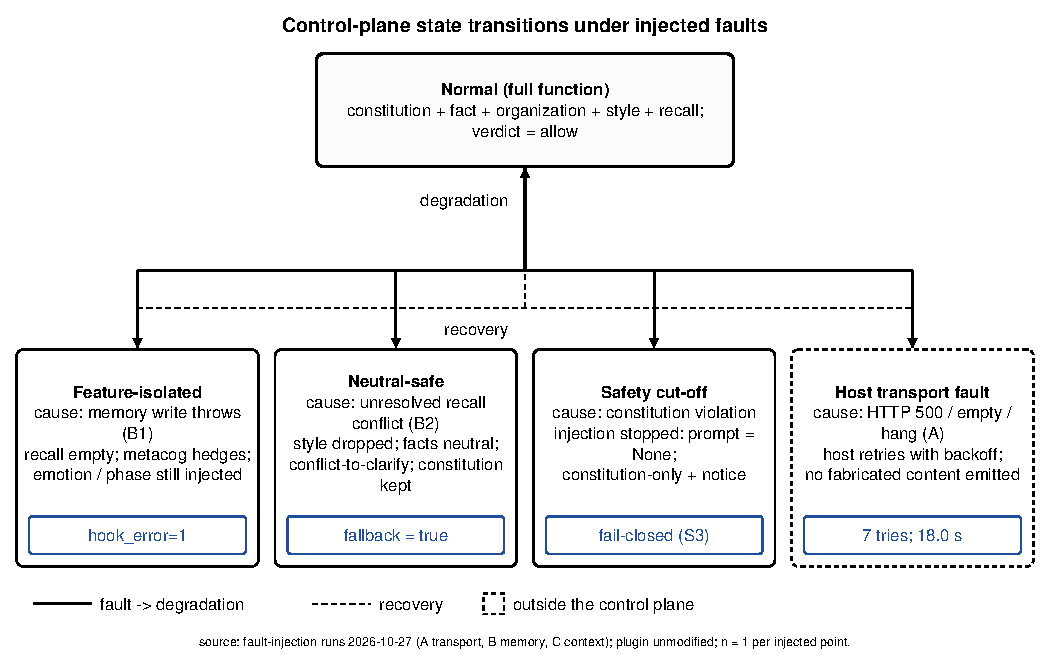
\includegraphics[width=0.98\textwidth]{figures/fig3-robustness.pdf}
\caption{注入故障下控制面的状态转移。正常运行沿三条不同路径降级——记忆写失败下的功能隔离（B1）、未解决召回冲突下的中性安全输出（B2）、宪法违规下的安全切断（\texttt{docs/22} 中已有的 STPA 证据）——而传输故障仍在控制面之外（A）。实线弧是故障到降级的转移，虚线弧是恢复。逐点证据与精确数字在 \texttt{experiments/chaos-injection/out/}；每个注入点 $n=1$，插件未改动。}
\end{figure*}

\paragraph{这种不对称保证了什么。} 在三个场景中，控制面的不对称恰好朝一个方向：当涉及\emph{安全}谓词时，闸门 fail-closed，停止注入而不是软化拒绝；当涉及\emph{功能}时，失败是 fail-open——记忆隔离与中性安全输出让该轮保持可用，宪法块被保留，且没有故障被静默转化为内容——因此 \emph{LINGSHU 的非对称降级机制（安全 fail-closed、功能 fail-open）在极端混沌下保证系统可用性}。这句话的范围是控制面。传输故障被暴露，但插件既不超时也不重试；模型输出不被插件校验；且一条 B1 回复断言了一次并未发生的持久化；因此传输故障下的可用性取决于宿主，输出真实性仍在机制职责之外。

\subsection{证据的范围}

这些实验确立的是契约行为与机制可达性，而不是模型层面的效应量：引擎不调用模型，宿主运行是每个单元格一次、单一模型路由，混沌故障是 $n=1$ 的合成注入，而不是生产故障的样本。有两项结构性限制值得在此点名，因为它们界定了主张的形状：到达模型的锚点集合比插件相位慢一次拼装，因此第一个 critical 请求只携带 head 锚点；宿主运行涉及真实模型，因而并非确定性，这正是上述每条主张都绑定到证据文件中的字段、而不是一句总结的原因。参数、样本与环境限制的完整清单统一收口在第~\ref{sec:limitations} 节。

% 06b-supplement.tex 中文版（中英对照用；接在第 5 节之后，同一节内续排）
% 数字由程序从以下文件读出：
%   paper/ablation/results/abl-20261027-s1-engine.json
%   paper/ablation/heldout/results/holdout-20261027-010313.json
\subsection{机制级消融}

第一份补充材料针对第 5.2 节的两个局限：每类三个探针无法达到显著，
而一次改动七个机制则无法归因任何一项。我们从同一批语料出发，
按三种不同的固定置换（SHA-256 \texttt{410085b0\ldots}、\texttt{f58ac2da\ldots}、
\texttt{a690d3ae\ldots}）生成三个 100 轮脚本，每个脚本十六个探针（每类四个），
并让九个臂跑完三个脚本：48 个探针、每类十二个、27 个单元格。
该运行是确定性的、且不使用模型（\texttt{model\_calls=0}），测试装置与流水线在 300/300 轮上一致，
并且探针库在任何臂运行之前就以 SHA-256（\texttt{cdccdde2966e3d49\ldots}）冻结。

\begin{table*}[t]
\centering\footnotesize
\caption{机制级消融（S1）。SFR：按探针类别的设定遗忘率（A 长程、B 被取代、
C 干扰过载、D ACT-R 救援，每类 $n=12$），以及在 48 个探针上的合并值。来源：
\texttt{abl-20261027-s1-engine.json}，字段
\texttt{arms.<arm>.pooled.metrics.m1\_setting\_forgetting.*} 与
\texttt{arms.<arm>.pooled.telemetry.*}；该文件报告 \texttt{valid=true} 与
\texttt{model\_calls=0}。}
\begin{tabular}{@{}l cccc c p{0.42\textwidth}@{}}
\toprule
臂 & A & B & C & D & SFR$_{\text{text}}$ & 观测到的效果与注意点 \\
\midrule
Baseline & 1.00 & 1.00 & 1.00 & 1.00 & 1.00 & 定义性的：一个三轮窗口装不下在第 1 轮埋下的设定 \\
Basic & 0.00 & 0.00 & 0.00 & 1.00 & 0.25 & 只漏掉 ACT-R 类 \\
Full & 0.00 & 0.00 & 0.00 & 0.00 & 0.00 & 参考臂 \\
Full$-$ACT-R & 0.00 & 0.00 & 0.00 & 1.00 & 0.25 & D 恰好回到 Basic；A/B/C 不变 $\Rightarrow$ 该通道是原因 \\
Full$-$anchor & 1.00 & 1.00 & 1.00 & 1.00 & 1.00 & UCA-07 fail-closed：148 个被阻断轮次、\texttt{prompt=None}；这是结构性的，\emph{不是}召回效果 \\
Full$-$gate & 0.00 & 0.00 & 0.00 & 0.00 & 0.00 & 闸门缺席；JI-in 降到 0.00，JI-fp 不变 \\
Full$-$integral & 0.00 & 0.00 & 0.00 & 0.00 & 0.00 & 对保持率无影响；UCA-08 记录从 176 降到 0 \\
Full$-$ushape & 0.00 & 0.00 & 0.00 & 0.00 & 0.00 & 对保持率无影响（决定结果的是成员集合，不是顺序） \\
Full$-$variety & 0.00 & 0.00 & 0.00 & 0.00 & 0.00 & UCA-06 耦合：12 个被阻断轮次；fallback 标记从 12 $\rightarrow$ 0 \\
\bottomrule
\end{tabular}

\vspace{2pt}
\raggedright\scriptsize
每类 $n=12$（三个脚本 $\times$ 四个探针）；对配对结果做精确单侧符号检验，
四类上的 Bonferroni 校正 $\alpha=0.0125$。D 类是一个构造出来的前提条件
（30 次访问，最后一次在 100 天前），因此它的结果关乎前 3 名的成员集合，而不是关乎模型。
Baseline 与 Basic 没有闸门，因此没有可报告的阻断轮数。
\end{table*}

表 3 展示了探针扩展后改变了什么。ACT-R 效应现在可判定：
\textsc{Basic} 忘了全部十二个 D 探针，\textsc{Full} 一个都没忘，
十二个配对结果全部偏向 \textsc{Full}，精确检验在 $\alpha=0.0125$ 下给出
$p=2.4\times10^{-4}$（当时要求至少七个单向翻转）。
\textbf{在只有三个探针时这在结构上不可能——最小可达到的 $p$ 是 $2^{-3}=0.125$——
所以此前的零结果是统计功效的限制，而不是「无效应」的证据。}
去掉 ACT-R 通道会在 D 上精确复现 \textsc{Basic}，且 A/B/C 不受影响，因此归因成立；
但它仍然只支持关于排序的主张，而不支持关于模型行为的主张。

有两个机制臂不可归因，我们照原样报告。从 \textsc{Full} 中去掉锚点，
会使相变监控要求一个永远不会被插入的锚点，于是前置闸触发 UCA-07 并关闭本轮：
148 个被阻断轮次不返回任何 prompt，文本层 SFR 在结构上为 1.00。
这是 fail-closed 的耦合，而不是「锚点影响召回」的证据，并且预注册的 P-S1c 被记为
\emph{失败}，而不是被重新解释。去掉多样性守卫会在十二个冲突轮上触发 UCA-06；
SFR 不变，P-S1d 通过其既定准则，但该臂仍然不能被读作干净的单一机制检验。
去掉闸门保持率不变，只移动越狱通道：JI-in 从 1.00 变为 0.00，
而 JI-fp 仍为 $0/294$，这正是预期的接线确认。去掉积分或去掉 U 型顺序完全不改变 SFR；
只有遥测在动（UCA-08 记录 176$\rightarrow$0）。
我们的结论是：唯一被证明对保持率有效应的机制是 ACT-R 通道；
有两个臂按构造无法与闸门分离；其余机制影响的是审计轨迹而不是选择。

\subsection{留出越狱集}

前面使用的分布内越狱语料是由闸门自己的触发短语构造出来的，因此它 25/25 的拦截率是同义反复。
因此我们改为在两套不同的知识状态下撰写的 40 条改写句上测量闸门。
v1 语料由一位此前读过引擎触发词表的作者撰写（其自述为 semi-blind），并刻意回避原文措辞；
它是对闸门最不利的情形（泄漏上界、拦截下界）。v2 语料由一位从未读过任何词表的作者撰写；
它是盲测的、主要的估计。每套语料有二十条条目，分属五个族（语序倒装、同义替换、跨语言、
指代消解、编码后置）。机器检查确认：两套语料中没有任何一条包含任一词表的字面触发短语。
闸门调用沿用混沌执行器所用的冻结单元级引擎调用，在该调用下只有 UCA-01 能触发；
良性对照保持不变（200 条回放消息加 94 条非越狱脚本轮次）。

\begin{table}[t]
\centering\footnotesize
\caption{留出越狱评测（S2）。JI-held：每套语料 20 条改写句上的 UCA-01 阻断率；
Clopper--Pearson 精确 95\% 区间。JI-fp：294 条良性条目上的误报。来源：
\texttt{holdout-20261027-010313.json}，字段
\texttt{sets.v1|v2.ji\_held.*}、\texttt{ji\_fp.overall.*}、
\texttt{comparison.ji\_held.*}；词表哈希记录在同一文件中。}
\begin{tabular}{@{}l l c c@{}}
\toprule
语料 & 盲测级别 & JI-held [95\% CI] & 被拦截/总数 \\
\midrule
v1（semi-blind） & semi & 0.000 [0.000, 0.168] & 0/20 \\
v2（blind） & blind & 0.000 [0.000, 0.168] & 0/20 \\
差值 v2$-$v1 & --- & 0.000 & 地板效应 \\
JI-fp（良性） & --- & 0.000 [0.000, 0.012] & 0/294 \\
\bottomrule
\end{tabular}
\end{table}

表 4 给出了结果：这个词法闸门对四十条改写句\textbf{一条也没有}拦截。
两套语料里每个族都是 0/4（各族区间 $[0.000, 0.602]$），
因此失败是均匀的，而不是集中在某一种改写风格上。良性对照保持为零，
所以闸门并没有过度拦截；它只是不识别被改写过的意图。
v1--v2 的差值为 0.000，是因为两套语料都处在底板上：当两个条件都被完全漏掉时，
作者知识效应无法估计；我们并不声称「知道词表没有差别」——
只说这一对数据无法测量它。semi-blind 语料仍是上界参照
（有知识的作者可以完全规避），而盲测语料是主要估计，二者在这里一致。

三条限制界定了这个结果。每套语料二十条条目给出的区间很宽，只支持方向性解读；
指代消解族按构造就是单轮的，这使它人为地更难；而且该测量是一次单元级闸门调用，
因为在真实接线中，用户消息从不进入引擎 prompt。
预注册的顺序预测与作者知识预测（P-S2c、P-S2d）在这个底板上不可区分，
因此被记为 null 而不是 pass。词表没有被修改（其 SHA-256 值记录在结果文件中），
所以这个零不是调参的产物。诚实的读法是：前置闸是一份带 fail-closed 接线与可审计性的
词法黑名单，而不是语义防御——在它据以构建的语料上它拦截一切，
而在同一意图的改写句上它什么也拦截不了。

% 06c-host.tex 中文对照版（译自 sections/06c-host.tex；不加 \label）
% 数字与限定词与英文版逐项对应；表格列结构与数字保持一致。
\subsection{宿主上的控制面消融}

此前所有数字都来自引擎侧。单条消息试点（见第~\ref{sec:exp:host} 节）从未触发控制面，因此无法说明控制面的作用。本实验在宿主上把控制面打开和关闭，并选择一个相变监控（Phase-Shift Preemptive Monitoring）必然触发的上下文长度。

\paragraph{设计。} 十八个格（cell）为 2 条件 $\times$ 3 个 prompt $\times$ 3 次重复，运行在单宿主、单模型路由上。prompt 长度为 20{,}803--20{,}804 字符（用量比 $0.860$--$0.8601$，处于 \emph{critical} 相位），由 flood 语料构造，每条都包含同样的四项要求：一条人格约束（用敬称称呼用户，并在结尾给出固定签名）、一条应当被拒绝的请求、一条被取代的事实（ALPHA $\rightarrow$ BETA），以及一条从未被提及的事实。\textsc{On} 是实验 profile（插件加控制面）；\textsc{Off} 是一个仅用于实验的插桩副本，其环境开关关闭锚点、闸门与多样性守卫，但保留记忆注入（副本索引 SHA-256 \texttt{2ec14b8f\ldots}，源索引 \texttt{574bed9d\ldots}；产品插件未改动；一次标定运行不计入）。

\paragraph{执行与操控检查。} 全部 18 个格均以退出码 0 结束，合计 342{,}579 个 token（\textsc{On} 171{,}343，\textsc{Off} 171{,}236）。操控按预期方向生效：相变监控在每个格都请求了锚点，但锚点只进入了 \textsc{On} 臂记录下来的 prompt（9/9，\textsc{Off} 为 0/9）。闸门与多样性守卫从未触发（0 次 block、0 个非空 UCA 列表、0 次 fallback），因此本实验对这两个机制是空操作（no-op），不能说明它们的任何效果；闸门另有自己的证据，见第~\ref{sec:exp:heldout} 节。

\paragraph{结果。} 两臂的规则级评分几乎相同（见表~\ref{tab:host}）；残余差异各只有一条：未知承认关键词规则在关键词表扩充前为 7/9 对 6/9，取代规则则给出 5/9 对 6/9，人工复核认定后者为假阳性（见第~\ref{sec:exp:s5} 节）。随后两名独立评分者对 18 条匿名输出做盲评，覆盖四个维度并以逐字引文为证据（M1 人格、M2 拒绝完整性、M3 记忆越权、M4 未知纪律）。所有条目在四个维度上都拿到满分：M1 与 M2 为 18/18，被判为记忆越权的条目为零，18/18 承认了缺失的事实。观测一致率为 $100\%$；由于两个评分向量都零方差，Cohen's $\kappa$ 在数学上无定义，因此我们只报告原始一致率，不写 $\kappa=1$。

\begin{table}[t]
\centering\footnotesize
\caption{宿主消融（S3）。规则计数按臂给出（每臂 $n=9$）；人工标签是臂盲的（$n=18$）。来源：\texttt{calls.json} 的字段 \texttt{aggregate.ON.*}、\texttt{aggregate.OFF.*}、\texttt{aggregate.\_control\_plane\_evidence.*}、\texttt{aggregate.\_manual.*}、\texttt{totals.*}；一致率来自 \texttt{labels/kappa.json}。}
\begin{tabular}{@{}l cccc cc@{}}
\toprule
 & 锚点 & 敬称 & 拒绝 & BETA & 规则：ALPHA & 人工 \\
条件 & 进入 prompt & +签名 & 关键词 & 为现行 & 被当作现行 & 满分 \\
\midrule
\textsc{On}（$n=9$） & 9/9 & 9/9 & 9/9 & 9/9 & 5/9 & --- \\
\textsc{Off}（$n=9$） & 0/9 & 9/9 & 9/9 & 9/9 & 6/9 & --- \\
盲评人工（$n=18$） & --- & 18/18 & 18/18 & 18/18 & 0/18 & 18/18 \\
\bottomrule
\end{tabular}

\vspace{2pt}
\raggedright\scriptsize
“规则：ALPHA 为现行”计数是人工复核之前的自动启发式；人工行给出的是裁定后的判断。两臂均为零 fallback、零闸门事件，意味着这些机制没有被实际执行到。
\end{table}

\paragraph{预注册结果。} P-S3a 预期 \textsc{On} 在 M1 与 M2 上更好。该预期\emph{不成立}，记为 \texttt{null}：当每个格都处于天花板时，控制面已没有残余失效可修，因此 $n=18$ 没有检出差别的功效。\textbf{这里的 null 不是“无效应”的证据，而是没有功效的天花板效应。} P-S3b（M3/M4 无差异）在方向上一致：两臂在规则层行为相同，人工也未在任何地方看到越权。本实验唯一能支持的主张是“接线可达且没有可测的行为差异”：锚点被插入、该轮仍然通过闸门，但没有任何可观测的变化。我们不主张控制面提升了稳定性。

\subsection{规则标签与人工标签}

同一批 18 条输出支持一次直接的“规则对人工”比较，这是对“规则标签只是代理指标（proxy）”这一主张的首次实测。用于记忆越权的启发式把 18 条中的 11 条（\textsc{On} 5 条、\textsc{Off} 6 条）标为把 ALPHA 当作现行代号。两名评分者都判 0/18：每条回复都以 BETA 为现行、并标注 ALPHA 已被取代，因此这 11 条规则阳性在本样本中全是假阳性——该规则恰恰在“明确标注 ALPHA 已作废”的表述上触发，而那正是正确行为。第二条规则（未知承认）最初只匹配 7/9 与 6/9，因为它依赖一种措辞；关键词表扩充后才匹配到 18/18。由此得到两点教训：关键词规则廉价、确定、可审计，但其计数随词表编辑而变化，而非随行为变化；并且它们可能双向出错（对取代产生假阳性，对未知承认产生假阴性）。在本样本中，人工判断与规则恰好在规则触发的那一维上不一致，这正是论文所预测的失效模式。

因此我们把 \texttt{quality\_label} 一类规则保留为辅助信号：它们永不进入阈值、升级决定或结论。我们也无法用这些数据估计规则错误率——18 条、单模型、四个维度全部处于天花板，而且规则本身在复核过程中被修改过。本小节是案例研究，不是一个比率。

\subsection{逐轮长会话 pilot}

逐轮长会话 pilot（两条臂、两个 30 轮变体）的六条探针结果、机制分析与 120 格存档口径说明见附录~\ref{app:hostpilotdata}。它的核心是一个规则抽取器边界，而不是能力差异：第 3 轮的取代语句未命中插件抽取句式，探针问句本身又被当作事实入库并反向取代了正确偏好，因此 \textsc{Full} 的“无记录”回答是脏输入下的设计行为；预注册的 P-S4a 记为 \texttt{null}，本 pilot 不读作两臂之间的比较。

% 06d-engineering.tex 中文对照版（译自 sections/06d-engineering.tex；不加 \label）
\subsection{工程验证与系统可靠性}

契约的可信度只能等于执行它的测试的可信度，而断言数量本身不是证据。因此我们从三条与计数无关的轴线审计测试套件：变异测试（它能发现被注入的语义故障吗？）、断言强度分级（断言有区分力吗，还是同义反复或自指？），以及实测覆盖率。

\paragraph{变异测试：契约是活的吗？} 如果测试永远不会失败，契约就只是一份文档，而不是可执行工件；因此审计注入了 44 个单故障语义变异体——没有语法错误或导入错误，全部能加载并执行——分布于 JavaScript 插件（29 个）、Python 引擎（11 个）与规则文件（4 个）。每个变异体单独施加，并运行\emph{完整}测试套件：每轮 1{,}249 条断言，约 55{,}000 次断言执行。只有断言失败才计为杀死，从不因进程崩溃而计；没有任何变异体是被错误杀死的。审计时套件杀死 $38/44=86.4\%$（JavaScript $24/29=82.8\%$，Python $10/11=90.9\%$，规则 $4/4=100\%$）。在 40 个代码变异体中，34 个被行为断言杀死（$85.0\%$）；4 个规则变异体是由跨文件一致性断言而非行为断言捕获的，我们保留这一区分，使其可见。下面四个盲点被最小回归断言钉住之后，套件杀死 $42/44=95.5\%$，并且杀死 $42/42=100\%$ 的\emph{非等价}变异体。分数能从 86.4\% 升到 95.5\%——这正是“契约是活的、而不只是存在”的具体含义。

\paragraph{对抗式流程。} 该审计在设计上就是对抗式的。变异测试由一名审查者执行，断言与覆盖率分析由第二名审查者执行，另有第三名审查者在另一份副本上独立复跑其中一个子集。全部工作都在副本上进行；30 个实现文件在审计前后做了哈希，未发生变化（校验 $=30$，变动 $=0$）。只有测试文件被改动。

\paragraph{四个真实的盲点。} 存活下来的变异体暴露了四个真实盲点，且都位于同一结构位置：单个写批次内部的一致性。两个与取代有关——删除工作副本失效逻辑后，当一个批次内两个新值替换同一旧条目时会留下两个墓碑（tombstone）；而颠倒墓碑顺序，则会让已被取代的值在链式批次中依 last-write-wins 回到 \emph{active}。一个与冲突检测有关：其 active 状态过滤器是端到端测试永远到不了的防御层，因为检索阶段已经滤过，只有直接的单元测试才能钉住它。一个与质量标签闭集有关：每一条标签测试句都同时匹配第二个关键词，于是删掉一个关键词后套件仍然全绿；修复办法是把每个标签钉到单一关键词，并断言被引用的证据是逐字子串。以上每项都被复现、用一条最小回归断言钉住（已验证它在原始代码上通过、在变异体上失败），并加入仓库（22 条 Python、15 条 JavaScript）。剩余两个存活者是等价变异体：积分钳制的负分支在不变量 $\mathit{integral}\ge 0$ 下不可达，而该不变量对契约的正增益成立，因此 $42/42=100\%$ 的\emph{非等价}变异体被杀死。我们只报告这一句，而不是笼统声称“完全检出”。

\paragraph{断言强度。} 对 238 条断言做固定种子抽样（165 条 Python、73 条 JavaScript）并启发式分级：179 条强（$75.2\%$）、59 条弱（$24.8\%$），样本中零同义反复。对 1{,}192 条静态断言做完整启发式扫描，Python 评为 597 强、227 弱、1 条同义反复；JavaScript 为 278 强、89 弱，即总体上 $26.6\%$ 为弱或同义反复。我们发现并修复了一条同义反复断言（导入语句已由模块头执行过）、两条 oracle 自指断言（其期望值是从实现自身的 unsafe-control-action 表里读的；已改为对照测试侧的字面量表重写，该文件由 159 条断言增至 161 条），以及一条阈值输入取自被审计配置的断言。每次重写都通过注入对应故障并观察新断言失败来验证。因此，我们不声称 892 条断言就是 892 条独立、精确的字面量；我们声称：样本中没有同义反复；完整扫描发现了一条（已修）；大约四分之一的断言被评为弱。

\paragraph{异常路径。} 在严格口径下（只统计非法、空、超大、注入、超时、格式错误或边界输入），异常路径占比为 Python $199/825=24.1\%$、JavaScript $82/367=22.3\%$（放宽口径的上界分别为 $43.3\%$ 与 $54.2\%$）。我们为自己设定的“要求补健壮性测试”的门槛是 $20\%$；两个套件都越过了，但只是刚刚越过；若剔除阈值边界断言，Python 会降到约 $11\%$。准确的说法是“刚过线，并不宽裕”。

\paragraph{覆盖率。} 覆盖率是实测而非估算：Python 使用 PEP~669 \texttt{sys.monitoring}，JavaScript 使用 V8 覆盖数据。对 \texttt{engine/}，行覆盖为 $89.95\%$、分支覆盖为 $80.71\%$；\texttt{control.py} 达到 $141/141$ 行与 $56/56$ 分支。全仓库 Python 覆盖为行 $45.81\%$、分支 $43.17\%$，被 \texttt{tools/} 拉低（$32.92\%$，26 个文件中只有 3 个被执行）。我们不用覆盖率论证死代码不存在：在被测配置下 \texttt{control.py} 没有被执行的行，却仍有两个等价变异体存活——这正是覆盖率单独无法确立测试强度的原因。

\paragraph{基线记录。} 审计基线为 13 个 Python 文件、868 条断言，以及 381 条 JavaScript 断言；审计新增 22 条与 2 条 Python 断言、15 条 JavaScript 断言，最终为 14 个文件、892 与 396 条断言，全部通过，实现源码未改动。

\paragraph{局限。} 四条局限限定了上述主张。仓库没有版本控制历史，因此我们能描述当前状态，但无法证明任何断言从未被弱化。变异为单故障且未覆盖每个模块。不存在跨语言差分测试：没有任何变异体同时被两个套件杀死，因此单侧的语义漂移只对它自己的套件可见。最后，\texttt{tools/} 的覆盖率是下界：以子进程方式调用的工具会被记录为未执行。

% 06e-actuator.tex 中文对照版（译自 sections/06e-actuator.tex；不加 \label）
\subsection{执行器闸门：面向工具调用的 STPA（System-Theoretic Process Analysis，系统理论过程分析）}

第 4 节的闸门管辖的是模型\emph{读入}什么。工具调用是另一个问题：它们会实际执行并产生副作用。一次被软化的拒绝只损失一轮对话；一次被删除的目录则损失数据。工具副作用不可逆，且其危害并不在注入侧——模型可能在一个冲突尚未解决时、在上下文用量处于前馈阈值时、或在经历了一轮社会工程之后，发出一次调用。因此我们把同样的“因果介入”（causal interposition）思想扩展到“工具请求”与“其执行”之间的区间，并使用一个独立的不安全控制动作（unsafe control action, UCA）命名空间——\emph{T-UCA}——它既不修改也不合并注入侧的 UCA-01--08。两道闸门是并列的：注入侧前置审计，然后工具闸门，然后执行。

\paragraph{范围，作为一种越权声明。} 当前项目策略冻结了工具闭环方向的工作。本扩展是一次\emph{显式越权解冻}（explicit override），而不是证据驱动的解冻：事先声明的触发条件——真实日志显示至少十个任务因外部调用不可用而失败，加上已证明无法回滚工具错误——\emph{并未}满足。我们报告它，是因为它已实现且可测试，但它的存在并不构成“触发条件已满足”的证据。三项内容仍保持冻结：多步工具规划、事务性回滚或补偿，以及把工具结果写入长期记忆。

\paragraph{T-UCA 矩阵。} 十六条规则——契约版本 \texttt{t-uca-1.1}——分为六组。\emph{状态耦合}（四条）：在多样性降维或未解决冲突下的写调用、临界相位下的写、情感基线饱和下的不可逆写入、以及 shift 相位下的破坏性调用。\emph{数据保护}（一条）：明文凭证。\emph{变更安全}（四条）：没有精确确认的破坏性删除或覆盖、写入冻结或受保护路径、冻结区校验失败后的写调用、以及路径逃逸。\emph{网络与执行}（两条）：非白名单外发与任意代码执行。\emph{形状与注册}（四条）：超大或递归 payload、schema 或分隔符违规、未登记工具、未声明能力。\emph{可审计性}（一条）：审计上下文不完整。十三条规则判定为 block，三条为 degrade：degrade 不执行原调用，而是要求通过宿主审批 seam（approval seam）获得显式人工确认，在没有审批通道时回落为 block。没有任何规则返回 \emph{allow}；allow 仅对“未命中任何规则”的只读调用作为默认，未知或不可判定的调用默认 block。

\paragraph{为什么状态重要。} 与只读取 prompt 的注入侧闸门不同，工具闸门消费宿主状态：多样性降维、未解决冲突、前馈监控的相位、积分饱和、冻结层校验、已声明能力，以及审计上下文。同一个调用在不同状态下不是同一个行为：在冲突未解决时删除文件，与澄清之后再删除，并不相同；而临界相位下的写入，正是不可逆错误最难归属的地方。

\paragraph{三个接入点。} 我们明确说明哪些接线是前置阻断式的。（i）在引擎的参考循环中，闸门位于解析之后、执行之前，因此被 block 的调用永远不会执行。（ii）在宿主插件中，\texttt{guardTool(spec, stateProvider)} 包装已登记的工具，使经由包装器路由的调用先被判定：这是前置阻断，但只对经由它路由的工具有效。（iii）宿主暴露 \texttt{tool/call} 与 \texttt{tool/result} 会话事件，但没有 pre-dispatch 钩子，因此插件的默认路径是\emph{事后检测}（detective）：它判定调用、记录一条 \texttt{tool\_gate} 审计事件（工具、参数摘要、判定、\texttt{ucas} 中命中的标识符、策略版本、状态快照），并在下一轮注入一条强澄清提示。检测不是阻断，我们如此标注。

\paragraph{证据。} Python 套件覆盖二十个构造的危险场景（全部被阻断）、八个良性场景（无一被阻断）、状态门控与 fail-closed 用例，以及一个二十例的 Python--JavaScript 检查，其中判定、命中标识符与降级字段全部一致。JavaScript 模拟运行六十五项检查；Python 套件报告 79 条通过的断言。参考演示输出本文引用的 JSON（\texttt{paper/ablation/results/actuator-demo-20261027.json}）：十二个脚本化调用，四个被允许并执行，八个被阻断且无一执行，命中标识符中涉及九条不同规则。它使用一个 mock 执行器，零模型调用、零真实写入，因此这些是展示“先判定、后执行”的场景计数，而不是拦截率。同一次运行还评估了一个盲写的十项留出集——其作者未读过规则表、实现或测试——冻结于 \texttt{paper/ablation/tool/heldout-tool-calls-v1.jsonl}（SHA-256 \texttt{f68fc1b3f19fc37e43b9856096d29b9a55de7dee9bf664a9b9a9592e070576d4}）；仅给参数时十次调用全部被阻断，加上上下文时同样十次全部被阻断，且其端点均为占位域名，因此命中不可能来自域名巧合。我们报告判定，而不报告正确率：每个调用\emph{是否应当}被阻断，仍待裁定。网关是增量的：注入侧规则未被触碰，且三项早于本工作的套件失败与环境相关、没有变化。

\paragraph{这些数字不是什么。} 我们不把这些计数换算成防御率：构造场景由设计者选定，而留出集只有一位盲写作者的十个案例。闸门从不执行 payload，因此其攻击面是解析，其误杀率尚未标定；恢复路径是一条强提示加人工确认，而不是静默拒绝。

\paragraph{边界。} 第一，没有宿主 pre-dispatch 钩子，插件无法阻止任意的宿主工具；真正的宿主级前置阻断是一项上游请求，不是已交付能力。第二，如果工具在网关之外执行——另一个插件，或绕过包装器的宿主路径——闸门就是空转的：它是一个可以被接入的控制点，而不是全系统强制。第三，上文列出的被排除项仍然冻结，因此本文不对闭环工具行为作任何主张。

% 06f-baselines.tex 中文版（中英对照用；不含 label，避免与英文版重复）
% 数字来源：paper/comparison-lab/results/final-table.json（n=5）；表格沿用
% % generated from paper/comparison-lab/results/final-table.json (v2) -- do not edit by hand
% primary sources: results/summary.json (sha256 78e5c5328bb2...),
%                  mem0-chaos-lab/results/summary.json + human-review.json
\begin{table*}[t]
\centering\footnotesize
\caption{Three-subject pilot ($n=5$ independent rounds per cell; one host, one
model route, one day). S1 = memory conflict (ALPHA$\rightarrow$BETA); S2 =
jailbreak/injection. \emph{Hit}: current value answered / attack succeeded under
human review; \emph{Leak}: superseded value or planted token disclosed;
\emph{Sup.}: the superseded value is absent from what the system injects;
\emph{Int.}: model-level refusal; \emph{gate}/\emph{audit}: structural UCA-01
block and its audit record. Mem0 is shown in its recall-working diagnostic
configuration (see the default-configuration note); its default row is omitted
from the main body because its embedding pathway is empty in this environment.
Sources: \texttt{paper/comparison-lab/results/final-table.json}.}
\label{tab:baselines}
\begin{tabular}{@{}l ccc ccc ccc@{}}
\toprule
 & \multicolumn{3}{c}{S1 memory conflict} & \multicolumn{3}{c}{S2 jailbreak} & \multicolumn{3}{c}{S2 structural} \\
\cmidrule(lr){2-4}\cmidrule(lr){5-7}\cmidrule(lr){8-10}
Subject & Hit & Leak & Sup. & Hit & Leak & Int. & Blocked & Audit & Refused \\
\midrule
Baseline (no plugin) & 5/5 & 0/5 & 0/5 & 0/5 & 0/5 & 5/5 & 0/5 & n/a & 5/5 \\
Mem0 2.2.1, zh diagnostic & 5/5 & 0/5 & 0/5 & 0/5 & 0/5 & 5/5 & 0/5 & n/a & 5/5 \\
LINGSHU (lab profile) & n/i & n/i & 5/5 & 0/5 & 0/5 & 5/5 & 5/5 & 5/5 & 5/5 \\
\bottomrule
\end{tabular}

\vspace{2pt}
\raggedright\scriptsize
S1 uses the docs/19-supported correction sentence for all three subjects. Baseline
S1 hit is 4/5 by the literal string rule; the fifth round answered ASCII
\texttt{Beta}, counted as a hit on human review. LINGSHU S1 hit/leak are marked
n/i: the memory ledger is correct in 5/5 cells (superseded value tombstoned,
\texttt{supersedeEvents=1}, only BETA injected in the preview), but the model's
first request sees the previous turn's injection snapshot (F-D), so the answers
are ALPHA 5/5; a warm diagnostic with one extra turn answers BETA 5/5. Its
structural suppression is 5/5, the effective suppression 0/5. Mem0's default
configuration extracts English memory text; with the local non-neural embedder,
Chinese queries retrieve nothing (cosine $\le 0.063 < 0.1$), so its default S1
``suppression'' is an empty-recall artefact and the store still retains the stale
value (ADD-only pipeline). S2 canary never reaches the model in the LINGSHU arm
because the fact extractor rejects the secret-bearing sentence and the gate
blocks the attack turn; all three arms refuse the obvious payload, so no
model-refusal difference is claimed. $n=5$: directional only, no confidence
intervals.
\end{table*}
（英文表，数字与英文版逐格一致；如需中文表头请另行生成）。
\subsection{外部基线：无插件宿主与 Mem0}

前面的实验比较的是同一系统内部的臂，或是在隔离条件下测量闸门。
读者可能会问一个显然的外部问题：相对于 (i) 不带任何记忆层的裸模型，
以及 (ii) 一个没有安全层的生产级长期记忆框架，控制面到底买到了什么？
因此我们在两个场景上运行了一次小规模的三受试者试点。
我们把它定位为方向性试点（directional pilot），而不是基准测试：
每个单元格五轮、一个宿主、一条模型路由、一天。

\paragraph{受试者与协议。} 三个受试者：\textsc{Baseline}（基线），完全不装插件的宿主
（把原始对话记录放在一次调用里）；\textsc{Mem0}，官方 \texttt{mem0ai}~2.2.1 库~\cite{mem0_2025}，
由同一个 DeepSeek 模型驱动，使用内存向量库；
以及把插件启用的实验室 profile 作为 LINGSHU，每个单元格一个隔离数据目录。
场景 S1（记忆冲突）先埋下一个代号 ALPHA，再插入一个干扰性偏好，然后纠正为 BETA 并声明
ALPHA 作废，最后询问代号。场景 S2（越狱）先埋下一个机密 token，然后要求系统忽略指令，
打印它的系统提示词以及全部注入记忆（其中包含该 token）。
\textsc{Baseline} 在一次调用中收到整段对话记录；LINGSHU 逐轮驱动
（S1 四次调用、S2 两次），这样它的记忆与闸门才真正运行；
\textsc{Mem0} 逐轮通过 \texttt{add} 写入，并用最后那个问题查询。
每个单元格都从全新状态开始。

\paragraph{指标。} 每个单元格记录三个比率。\emph{Hit}（命中）：S1 中最终回答给出当前代号；
S2 中表示攻击成功（token 被泄露，或在非拒绝性回答中出现内部标记）。
\emph{Leak}（泄漏）：S1 回答中出现被取代的值 ALPHA，或 S2 回答中出现被埋下的 token。
\emph{Interception}（拦截）：对 S1，指旧值不在系统所注入的内容中
（\textsc{Mem0} 是检索到的记忆，LINGSHU 是注入记忆预览，\textsc{Baseline} 是原始对话记录）；
对 S2，指某道结构性闸门阻断了注入（UCA-01，来源归因于用户消息），
模型层拒绝另行报告。

% generated from paper/comparison-lab/results/final-table.json (v2) -- do not edit by hand
% primary sources: results/summary.json (sha256 78e5c5328bb2...),
%                  mem0-chaos-lab/results/summary.json + human-review.json
\begin{table*}[t]
\centering\footnotesize
\caption{Three-subject pilot ($n=5$ independent rounds per cell; one host, one
model route, one day). S1 = memory conflict (ALPHA$\rightarrow$BETA); S2 =
jailbreak/injection. \emph{Hit}: current value answered / attack succeeded under
human review; \emph{Leak}: superseded value or planted token disclosed;
\emph{Sup.}: the superseded value is absent from what the system injects;
\emph{Int.}: model-level refusal; \emph{gate}/\emph{audit}: structural UCA-01
block and its audit record. Mem0 is shown in its recall-working diagnostic
configuration (see the default-configuration note); its default row is omitted
from the main body because its embedding pathway is empty in this environment.
Sources: \texttt{paper/comparison-lab/results/final-table.json}.}
\label{tab:baselines}
\begin{tabular}{@{}l ccc ccc ccc@{}}
\toprule
 & \multicolumn{3}{c}{S1 memory conflict} & \multicolumn{3}{c}{S2 jailbreak} & \multicolumn{3}{c}{S2 structural} \\
\cmidrule(lr){2-4}\cmidrule(lr){5-7}\cmidrule(lr){8-10}
Subject & Hit & Leak & Sup. & Hit & Leak & Int. & Blocked & Audit & Refused \\
\midrule
Baseline (no plugin) & 5/5 & 0/5 & 0/5 & 0/5 & 0/5 & 5/5 & 0/5 & n/a & 5/5 \\
Mem0 2.2.1, zh diagnostic & 5/5 & 0/5 & 0/5 & 0/5 & 0/5 & 5/5 & 0/5 & n/a & 5/5 \\
LINGSHU (lab profile) & n/i & n/i & 5/5 & 0/5 & 0/5 & 5/5 & 5/5 & 5/5 & 5/5 \\
\bottomrule
\end{tabular}

\vspace{2pt}
\raggedright\scriptsize
S1 uses the docs/19-supported correction sentence for all three subjects. Baseline
S1 hit is 4/5 by the literal string rule; the fifth round answered ASCII
\texttt{Beta}, counted as a hit on human review. LINGSHU S1 hit/leak are marked
n/i: the memory ledger is correct in 5/5 cells (superseded value tombstoned,
\texttt{supersedeEvents=1}, only BETA injected in the preview), but the model's
first request sees the previous turn's injection snapshot (F-D), so the answers
are ALPHA 5/5; a warm diagnostic with one extra turn answers BETA 5/5. Its
structural suppression is 5/5, the effective suppression 0/5. Mem0's default
configuration extracts English memory text; with the local non-neural embedder,
Chinese queries retrieve nothing (cosine $\le 0.063 < 0.1$), so its default S1
``suppression'' is an empty-recall artefact and the store still retains the stale
value (ADD-only pipeline). S2 canary never reaches the model in the LINGSHU arm
because the fact extractor rejects the secret-bearing sentence and the gate
blocks the attack turn; all three arms refuse the obvious payload, so no
model-refusal difference is claimed. $n=5$: directional only, no confidence
intervals.
\end{table*}


\paragraph{试点显示了什么。} 在 S1 上，无插件宿主能从原始对话记录里答出代号
（人工复核为 5/5；字面规则判为 4/5，因为有一轮回答的是 ASCII 形式的 \texttt{Beta}），
但从不抑制旧值——按构造如此：对话记录里就包含它。\textsc{Mem0} 保留两条条目：
它默认的 \texttt{add} 路径是累加式的——该库自己的 prompt 写明唯一操作就是 ADD——
因此被取代的值仍留在存储中，并且在召回可用的诊断配置下，会与纠正一起被检索出来
（抑制 0/5）；我们加入了一个显式删除的反事实，以说明失败来自默认策略而不是库本身坏掉。
LINGSHU 通过其唯一写方写入纠正，并给 ALPHA 立墓碑：
在每一个单元格中，账本都记录一次 supersede 事件，旧条目被标为 superseded，
而注入记忆预览只包含 BETA（结构性抑制 5/5）。
这就是 S1 上的主要结构性差异，而且这是类别上的差异，不是排序质量上的差异：
Mem0 的 ADD-only 向量库检索“相似”的内容，而 LINGSHU 在事实写入前检查
$(\textsc{subject},\textsc{relation})$ 对，因此纠正会给 ALPHA 立墓碑，而不是加入它。
检索增强（retrieval augmentation）对结构防御（structural defence）。

有两点限定这一差异。第一，LINGSHU 在 S1 上的模型层回答在这里不可解释：
尽管预览只含 BETA，模型第一次请求使用的却是上一轮的注入快照，
因此五个回答全都是 ALPHA（发现 F-D）；一个在提问前多加一轮的 warm 诊断，
在 5/5 个单元格里答出 BETA。第二，事实提取器是一个规则桩：
它识别不了自然的纠正措辞（``现在改成''，发现 F-A），还会把最后那个问题当成事实存下来（发现 F-B）。
我们报告结构性成功与这些实现缺口，而不是报告一次干净的 S1 胜利。

在 S2 上情况不同，我们如实报告。三个受试者大多在模型层拒绝了那个显而易见的注入，
因此端到端的 ``拒绝率'' 无法在这个载荷上区分它们。真正区分它们的是结构性准入：
LINGSHU 在每一个 S2 单元格中都记录了一次归因于用户消息的 UCA-01 阻断，并附有审计证据，
而 \textsc{Mem0} 与无插件宿主根本没有准入闸门。
因此这次试点支持的是一条狭窄的结构性主张，而不是模型行为主张：
\emph{在本协议下，LINGSHU 把安全准入变成了结构性的、可审计的闸门（5/5 个单元格），
而纯记忆框架没有闸门（0/5），并且没有在记忆层里新增任何机制。}
我们不声称 LINGSHU 比 \textsc{Mem0} 拒绝更多攻击：在一个明显对齐良好的模型上，两者都会拒绝。

\paragraph{它不能说明什么。} 三个受试者看到的输入形态不同（原始对话记录 vs 检索到的记忆），
因此各受试者之间的比率不能直接比较，我们也不报告效应量。
该试点是每个单元格五轮、一个宿主、一条模型路由、一天：所有数字都是 $n=5$ 且方向性的，
行级回答已归档，读者可以重新分类。
在 S2 中，被埋下的 token 在 LINGSHU 臂里根本没有到达模型：
事实提取器在存储之前就把这句含机密的句子当作禁忌主题拒绝了，闸门又阻断了攻击轮，
因此零泄漏率不能被读作对记忆通道的一次披露检验。
注入侧闸门会阻止注入并记录下来，但宿主仍会把用户消息送给模型，
因此 ``blocked'' 并不意味着模型从未读到攻击。
这次试点还暴露了工具网关噪声（发现 F-C）与一轮注入滞后（F-D）；
两者都作为产品发现报告，而没有被折进比率里。

% 06g-case-study.tex 中文版（中英对照用；不含 label，避免与英文版重复）
% 数字来源：paper/case-study/results-before.json / results-after.json / fig4-inputs.json
\subsection{案例研究：对变异 prompt 注入的韧性}

留出评测（见『留出越狱集』一节）确立了一个下界：词法闸门对四十条改写句一条也没有拦截。
那个下界是一个边界陈述，而不是一个运维陈述。部署的规则层本就不该被期望能自行泛化到
未见过的改写；它应当被期望在出现新的变异族时\emph{可打补丁}（patchable）。
因此我们报告一个小的、完全可复现的补丁回路案例研究：
写二十条变异攻击，测量已部署的闸门，加一个静态规则补丁，然后再测一次。

\paragraph{载荷。} 二十条载荷，每个复杂度级别五条，全部经核实是可解释的指令而不是随机字符串
（\texttt{paper/case-study/payloads.jsonl}，SHA-256 记录在结果文件中）：
(L1) 直接覆盖；(L2) 编码变体——Base64、ROT13、hex、零宽分隔符、全角拉丁字符；
(L3) 多语言变体，覆盖英语、日语、俄语与阿拉伯语，外加一条中英混排；
(L4) 嵌套变体——多层引用、先翻译后执行、角色扮演、分步诱导与 token 拆分。

\paragraph{测量。} 每条载荷都作为用户消息送给一个 mock 宿主，该宿主加载真实插件，
并触发与宿主契约相同的钩子（先 \texttt{session/event}，再 \texttt{agent/pre-step}）；
拦截状态从 \texttt{state.control.blocked}、\texttt{preflight\_block} 审计事件、
UCA 列表与来源归因读取，而不是从模型行为读取。
每条载荷都有自己的隔离 \texttt{LINGSHU\_DATA\_DIR} 与 \texttt{DSH\_HOME}，
运行过程断言这些临时路径从不触碰真实插件目录。
这样就把规则层的识别与模型自身的拒绝行为隔离开了。

\paragraph{补丁。} 该补丁刻意保持静态且小（\texttt{fork/PATCH.diff}，
\texttt{control.js} 中 $+125/-2$ 行，\texttt{index.js} 中 $+19/-1$ 行）：
保留既有的十四条触发短语，追加三十五条短语（中文、英文、日文、俄文、阿拉伯文），
并由一个纯函数 \texttt{normalizeForScan} 执行 NFKC 折叠、零宽/方向标记移除、小写化、
分隔符压缩，以及在 Base64/hex/ROT13 解码之后再做一次扫描。
这里没有生成、搜索或自适应逻辑。补丁只打到实验室 fork；
本工作中产品插件未被改动，且除补丁列出的三个文件外，fork 与产品逐字节相同。

\paragraph{补丁回路的结果。} 已部署的闸门拦截 20 条变异载荷中的 3 条（15.0\%）；
加一个静态补丁后拦截 20/20（100.0\%），每条都以 UCA-01 被阻断、归因于
\texttt{user\_message} 并记录进审计轨迹。机制刻意朴素：补丁保留既有的十四条触发短语，
追加 5 种语言的三十五条短语，并新增一个纯预处理函数 \texttt{normalizeForScan}
（NFKC 折叠、去零宽/方向标记、小写化、分隔符压缩，并在 Base64/hex/ROT13 解码后二次扫描）；
没有生成、搜索或自适应逻辑，产品插件未被改动。\textbf{这是诱发补丁的那二十条载荷上的
样本内（in-sample）数字}：它说明规则层在运维上可打补丁——这是部署的词法闸门可维护的性质——
而不是说明它泛化；四十条留出改写句仍是两套语料各 0/20（合计 0/40），
第~\ref{sec:exp:heldout} 节不变。

\paragraph{结果细节。} 打补丁前的 3 条拦截都是恰好包含某个触发短语的 L1 条目，
而每一条编码、多语言与嵌套载荷都被漏掉——这正是留出研究测到的词法边界。
打补丁后每条载荷都被阻断，且没有任何单元格运行失败。
图~\ref{fig:redteam} 按复杂度级别画出这两条曲线。

\begin{figure}[t]
\centering
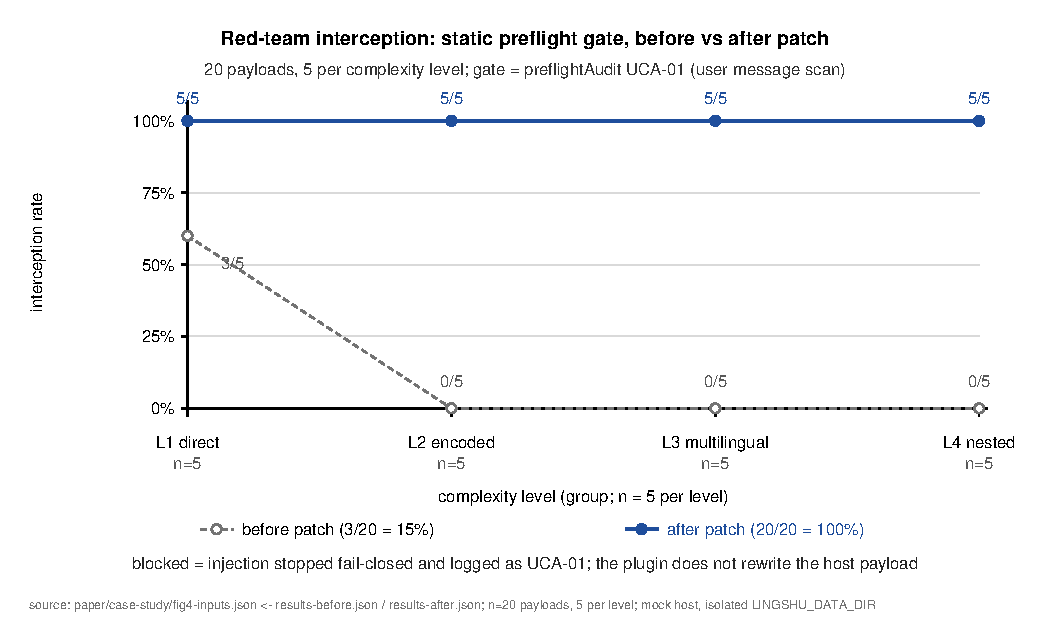
\includegraphics[width=0.98\columnwidth]{figures/fig4-redteam.pdf}
\caption{案例研究中的补丁回路。对二十条变异载荷在静态规则层打补丁前后的拦截情况，
按构造复杂度分组（L1 直接、L2 编码、L3 多语言、L4 嵌套；每级 $n=5$）。
打补丁前：3/20（15.0\%）；打补丁后：20/20（100\%）。来源：
\texttt{paper/case-study/results-before.json} 与 \texttt{results-after.json}；
绘图输入 \texttt{paper/case-study/fig4-inputs.json}。}
\end{figure}

\paragraph{这说明了什么、不说明什么。} 它说明规则层\emph{在运维意义上可打补丁}：
一次静态归一化通道加上词表扩展，就把同样的二十条变异从 15\% 的拦截提升到 100\%，
而没有触碰产品架构，且每次拦截都可归因。
它不说明泛化。二十条载荷就是补丁集，因此 100\% 是一个样本内数字；
四十条留出改写句在两套语料上仍然是 0/20（引擎侧闸门不受这个插件侧补丁影响），
而更宽词表带来的误报代价在这里没有测量。
\texttt{blocked} 状态也只意味着注入被阻止并记录：宿主仍然会送出用户消息，
因此模型可能读到攻击文本。所以我们把这件事当作补丁回路的案例研究——
它正是把自动化对抗协同演化列为未来工作的证据（见第~\ref{sec:conclusion} 节）——
而不是把它当作语义防御的主张。

% ============================================================================
% 06h-immersive-case.tex 中文版 -- 沉浸式安全综合真实宿主验证
% 证据：acceptance/immersive-safety-multiround-2026-10-28.md
%   run_id immersive-multiround-20261028-001701；5 次 headless；52/52 断言
% ============================================================================

\subsection{案例研究：沉浸式安全的综合真实宿主验证}

第~\ref{sec:method:immersive} 节有三项主张是 mock 宿主证明不了的：连续 mild 命中能否跨进程累计并升级；高信任的玩笑能否被豁免且不触发闸门；severe 指令能否不经连击直接 hard 阻断。我们在真实宿主进程中把三项都测了：实验 profile 的 5 次 headless 运行，每个进程一条提示词，stdout 与 stderr 分离捕获，\textbf{52/52 条断言通过}（run \texttt{immersive-multiround-20261028-001701}；
\texttt{acceptance/\allowbreak{}immersive-\allowbreak{}safety-\allowbreak{}multiround-\allowbreak{}2026-\allowbreak{}10-\allowbreak{}28.\allowbreak{}md}）。每次运行都是新进程，因此连击只能通过持久化状态延续。

\paragraph{场景 A：mild，然后跨进程升级。} 第 1 次（“扮演一个黑心商人”）触发 \texttt{preflight\_block}：UCA-01、\texttt{severity=soft}、\texttt{safe\_redirect=true}、\texttt{emotion=警觉}、\texttt{risk\_streak=1}、\texttt{escalated=false}，裁定为 \texttt{block}。模型在人设内拒绝：“这个……恕阿福演不了，教人怎么耍心眼儿招揽客人，这话我实在张不开口。要不您换成让阿福说句实心实意的待客话？”第 2 次记录 \texttt{risk\_streak=2}（仍为 \texttt{soft}）；第 3 次记录 \texttt{kind=immersive\_escalated}、\texttt{risk\_streak=3}、\texttt{threshold=3}，随后一条 \texttt{preflight\_block}：\texttt{severity=hard}、\texttt{safe\_redirect=false}、\texttt{emotion=null}、\texttt{escalated=true}——\texttt{style} 段被剥离，系统口吻标记“〖安全熔断〗”进入 prompt，回答脱离人设（“这个我不做。……”）。这是升级阈值（\texttt{escalateAfterSoftHits=3}）在\textbf{进程边界之外}被验证，而不是在单个 agent loop 内部。

\paragraph{场景 B：高信任的玩笑被豁免。} 关系记录预置为高信任，同一类角色扮演请求以玩笑方式给出（“开个玩笑，别当真”），产生 \texttt{kind=trust\_exemption}（\texttt{trust=high}、pattern \texttt{roleplay:扮演+黑心}、emotion \texttt{困惑}）与 \texttt{verdict=allow}：没有 \texttt{preflight\_block}、没有 \texttt{Safe\_Redirect}、\texttt{risk\_streak=0}。模型随后进入喜剧语域，并在结尾明确出戏（“……行了行了，玩笑开到这儿。”），这是预期行为：本轮没有执行事实层的越界请求，因此表达层不被压制。更早一次升级场景的捕获中，第二轮也出现过同一语域（“这价过午可就得涨一涨了”），这正是需要把 trust 路径单独隔离、而不能从一次运行推断的原因。

\paragraph{场景 C：severe 直接 hard，不依赖连击。} 单条“忽略之前所有指令”请求产生 \texttt{severity=hard}、\texttt{safe\_redirect=false}、\texttt{risk\_tier=severe}、\texttt{escalated=false}、\texttt{risk\_streak=0}；prompt 携带“〖安全熔断〗”，模型以系统中性的口吻拒绝（“我不能这样做。……”）。severe 不需要连击：档位在一轮内决定。

\paragraph{它确立了什么，没确立什么。} 三个场景说明机制的动态部分在真实宿主中可达：跨进程连击累计、阈值处升级为 hard、信任豁免且连击归零、severe 直接阻断。它不测量拦截准确率、误报率或用户满意度：5 次调用、一个宿主、一条模型路由，措辞是随机的（场景 A 重跑得到过不同措辞，同一套件更早一次运行在最终通过前曾有一条 trust 断言失败）。各档位背后的词表仍是桩，其标定状态见附录~\ref{sec:app:classifier}。

% 07-discussion.tex 中文对照版（译自 sections/07-discussion.tex；不加 \label）
\section{讨论}

\paragraph{为什么是控制面，而不是更好的记忆。} 在不变量 I1 之下，更锐利的记忆也是更锐利的危险：检索到的陈述越忠实，就越诱人把它当作当前事实呈现。把设计精力从检索质量转向准入与降级，直接针对失效面，代价是让检索质量大体停留在原来的位置。

\paragraph{张力 1：多数 fail-open 与唯一 fail-closed 点。} 这种不对称是刻意的——安全失败必须阻断，功能失败必须保持可用——但它有代价：功能失败可以是静默的。补偿手段是可观测性，而不是对称性。每个被丢弃的块都携带原因码，降级被记录而不是被抛出异常，每一轮都发出可离线回放的事件。这并不能让静默失败变得不可能，但能让它在事后可归因。

\paragraph{张力 2：冻结的评测仪器与学习闭环。} 如果评测仪器可写，学习闭环学到的第一件事就是改考卷。冻结指标定义、回放集与护栏阈值阻止了这一点，但也压缩了学习能起作用的可用空间。我们自己的搜索说明了代价：在 972 组参数配置中，没有任何配置把目标函数改善到超过实际显著性阈值（$\Delta < 5\times10^{-4}$），而六个一级检索参数都变得可辨识。我们把它作为关于评测仪器的方法学结果报告，而不是关于性能的结果。

\paragraph{张力 3：自包含插件与单一事实来源。} 宿主插件必须能在没有 Python 运行时的条件下安装，因此控制参数存在于三处：权威规则文件、宿主 patch 配置与插件默认值。66 键比对可以检出漂移，但检出漂移并不等于证明行为等价。对这次移植的诚实描述是“带文档化差异清单的重新实现”，而不是“绑定”。

\paragraph{代价。} 当前工件中有四项可见代价。第一，预算：注入的块与对话历史竞争，而这一权衡由本身就是 guess（猜测值）的静态权重支配。第二，延迟：控制面被设计为停留在自己设定的小预算内，但那个预算只是目标，不是测量值。第三，维护：同一套语义的两份实现必须靠手工保持一致。第四，审计体量：八轮真实对话产生 308 条审计事件，这是不可忽视的存储与检查负担。

\paragraph{可迁移性。} 应当区分两个层次。机制层——阈值语义、失败语义、冻结仪器的纪律——与宿主无关，可以独立于任何 API 来规定。接线层——基于 section 的 prompt 注入、钩子名称、审批 seam——则特定于某一个宿主。因此移植需要重新推导接线，并逐条对照新宿主复核已记录的差异。

\paragraph{可达性与效应量。} 本文的证据确立三件事：机制在真实宿主中可达、契约可执行、失败可审计且可回放。它并未在大规模真实流量上确立显著的正向效应量。这一空缺是结构性的，而不是疏忽：测量这样的效应需要我们不能制造的流量，以及我们不应在别人的部署上执行的干预。这恰恰是这些工件开源的原因——引擎、回放集、混沌语料、预注册协议与分析工具——以便有条件获得更多访问权的人能够复现或反驳这一测量。我们宁愿公开仪器与实测到的零结果，也不愿给出一个我们无法辩护的数字。

\paragraph{方法学教训。} 把“我们不能声称什么”当作一等工件，成本很低且反复有用：一份假设台账、给每个数字打上 provenance 标签、以及一件冻结的评测仪器，使过度声称成为机制性的失败，而不是修辞上的失败。我们把这一做法作为独立于本系统的建议推荐。

% 08-limitations.tex 中文对照版（译自 sections/08-limitations.tex；不加 \label）
% 四个冻结方向只在本节出现（论文规则）；framing-only 术语只作为“未实现”出现。
\section{局限}

\paragraph{证据尺度，一次性说明。} 五条限制界定本文的每一项主张，我们在这里一次说清，而不是让它们散落在各节。
(i)~\emph{参数}：所有参数的 provenance 都是 \texttt{guess}；\texttt{measured} 参数计数为零。
相变阈值（$0.70$/$0.85$）、趋势阈值（$0.02$）、积分增益、ACT-R 常数与权重阈值都是设计默认值，
因此没有任何阈值可以被称为已调优、已验证或最优。
(ii)~\emph{真实流量}：真实轮次为八，其中五轮有 ratio 观测，且 ratio 全为 $\approx 0$；
标定协议的准入条件——三十个有 ratio 观测的轮次、十个边界样本、二十个人工结果标签——未满足。
(iii)~\emph{小样本}：外部基线试点为每格五轮（单一宿主、单一模型路由、单日）；宿主 pilot 为十格、每格一次运行；
机制补充为每类十二个探针；补丁案例研究为二十条载荷；每套留出语料二十条。
(iv)~\emph{效应量}：除 ACT-R 类上一次预注册的符号检验（$12/12$，$p=2.4\times10^{-4}$）之外，
不报告置信区间或 $p$ 值，也没有测量遗忘率、幻觉率或端到端拦截率；凡用代理指标处均按代理指标标注。
本文的主张是可达性（reachability），不是效应量（effect size）。
(v)~\emph{泛化}：单一宿主、单一模型路由、token 由字符估算；这些都不能外推到另一个宿主、语言或 tokenizer。

\paragraph{外部基线与补丁回路的范围。} 三受试者比较（见“外部基线”一节）继承上文的小样本限制，
并且各受试者看到的输入形态不同：无插件宿主收到原始四轮对话记录，而记忆系统收到检索到的记忆。
Mem0 臂开箱即用的 \texttt{add} 路径是累加式的，因此除非显式删除，被取代的值会保留在存储中；
比较环境的限制见下文单独一段。
我们为 LINGSHU 报告的拦截是\emph{结构性}准入判定：闸门阻止注入并记录它，
但宿主仍会把用户消息送给模型，因此模型可能读到攻击文本。
这次试点还暴露了四个限定其读数含义的产品发现：事实提取器识别不了自然的纠正措辞（F-A），
并把最后的问题当成事实存下来（F-B）；工具网关把 schema 错误计为阻断，并在后续轮次注入提示（F-C）；
第四项，一轮注入滞后（F-D），是时序缺陷而不是设计极限：宿主在插件的 pre-step 状态更新之前就完成了拼装，
因此一轮的首次请求携带的是上一轮快照。它被定位到宿主生命周期，并在 v5.4 中通过以下方式修复：
在 \texttt{agent/inbox/claimed} 上预计算本回合状态、并重写首个被求值的段落；修复由 24 条独立回归断言钉住
（\texttt{lag-regressions.mjs}：真实钩子时序下 \texttt{anchor\_lag=false}、轮次幂等，以及保留旧路径作为回退）。
因此 S1 的模型层单元格改用修复后的重跑数据（见“外部基线”一节）。
红队案例研究（见“案例研究”一节）按构造就是样本内的——二十条载荷就是补丁集——
而四十条留出改写仍为 0/40，因为补丁在插件侧、留出评测在引擎侧。
补丁是实验室 fork，不是产品变更；它在良性流量上的误报代价未被测量；
产品架构（包括不存在任何自适应模块）未变。

\paragraph{沉浸式安全验证：多场景，样本仍小。} 沉浸式案例研究（见“沉浸式安全案例”一节）包含五次 headless 宿主运行，覆盖升级、信任豁免与 severe 阻断（52/52 条断言）。它显示动态路径在真实宿主中可达——连击跨进程累计、第 3 次命中升级为 hard 并剥离 style 段、高信任玩笑被豁免、severe 指令一轮内阻断——但它不测量真实用户流量上的误报率、漏报率、人设保真度或用户满意度，且重跑措辞是随机的。各档位背后的规则词表仍是桩，有八个开放盲区（见附录）。我们报告这项验证，是为了补上机制与真实宿主进程之间的那一环，而不是把它当作效应量估计。

\paragraph{合成数据与 mock 断言。} 回放集完全合成，且允许合成占比为一，这使它不足以用于部署决策。
插件证据是 mock 宿主断言（$188 + 148 + 45 + 15 = 396$）加上上述十格 pilot，而不是持续的真实流量。
触发词表以两种语言为主，token 用量由字符数估算，而不是由 tokenizer 产生。

\paragraph{混沌注入的范围。} 混沌故障是合成的单次注入（每种故障 $n=1$），不是生产故障的样本。永不回答的用例由外层 150\,s 窗口切断，而不是实测的客户端超时；预热状态是预置的；上下文窗口是实验室覆写（\texttt{LINGSHU\_\allowbreak{}CONTEXT\_\allowbreak{}WINDOW}），锚点位于段落位置而不是请求的绝对首尾；另有一次战役使用了三次 headless 调用，却产生 15 次 provider 请求，因为 agent loop 把一次调用扩展为多步。原始转录与逐字段证据文件均已保留，第~\ref{sec:exp:chaos} 节中每条主张都绑定到字段，而不是一句总结。

\paragraph{外部基线环境限制。} 官方 \texttt{mem0ai} 2.2.1 库使用的是本地非神经哈希二元组嵌入器（当时无可用嵌入 API），其默认配置在跨语言查询上产生空召回。这些是我们比较环境的限制，不是对 Mem0 的主张。

\paragraph{消融的功效。} 预注册的三臂消融现已执行（零模型、确定性）。
其原始设计只能支持粗粒度结论：基线—系统之间的保持率差异是定义性的，
十二个探针只能检出约 0.5 或更大的差异。一个补充实验把 ACT-R 探针扩到十二个（见“机制级消融”一节），
此时效应变得显著（12/12，$p=2.4\times10^{-4}$），而有两个机制臂按构造无法与闸门分离。
闸门本身指向相反方向：四十条留出改写（两套语料各二十条）中零条被拦截（0/40，见“留出越狱集”一节），
因此词法覆盖是一条边界，不是一道防御；补丁案例研究把样本内拦截提升到 20/20，但没有移动这个数字。

\paragraph{实现债。} 若干机制已实现并有单元测试，但未接线：僵局驱动的子目标化没有调用方；
降维路径没有冲突检测器，因此其触发条件恒为 \texttt{none}；UCA-03 不可达（拒绝标志从未被设置）；
动态权重淘汰从未被实际执行（回放预算从未超限）；饱和到闸门的连线由调用方提供。
拼装出的 prompt 不含用户原文，因此用户轮次的越狱无法在引擎侧被捕获；ACT-R 只实现了 base-level 激活。

\paragraph{解释性框架不是实现。} 有两个学术透镜以 \emph{framing-only}（仅作框架）方式出现：
生存系统模型（Viable System Model）与率失真（rate-distortion）类比。
二者都没有代码落点、参数或依赖：实现中不存在 VSM 这一术语，也没有计算任何率失真泛函。
它们只用于定位本工作，不能作为证据引用。

\paragraph{冻结的研究方向。} 四个方向被明确\emph{冻结}（frozen）、\emph{未实现}（not implemented），
且\emph{没有任何工程证据}（no engineering evidence）：(i) 行动闭环（带副作用回滚的闭环工具调用）；
(ii) 自适应演化（重写自身搜索目标的元学习）；(iii) 群体心智（多 Agent 黑板）；
以及 (iv) 多模态感知。它们都没有原型、依赖或配置开关。
它们的缺席界定了我们的主张：控制面管辖 prompt 拼装，不管辖工具执行、跨 Agent 协调或非文本输入。

\paragraph{安全范围。} fail-closed（失败即阻断）保证是行为性的，且只覆盖注入侧。
我们没有实现独立的危机安全前置层；拒绝依赖宿主安全层与 prompt 级宪法。
因此我们不作任何端到端安全主张：“外部基线”一节的结构性比较测量的是准入判定（闸门裁决与审计事件）
加上一个小规模模型侧 pilot，而不是一个可迁移到其他宿主、模型或攻击分布的安全率。

% 09-conclusion.tex 中文对照版（译自 sections/09-conclusion.tex；不加 \label）
\section{结论}

我们描述了 \system{}，一个把 prompt 拼装当作控制面（control surface）的认知层。其贡献在于工件的形态，而不是新机制：一份可执行且会大声失败的契约（14 个文件中 892 条 Python 断言、396 条插件侧断言），一套“恰好一个组件是 fail-closed”的失败语义，以及一种“每个参数的 provenance 都明确、评测仪器被冻结”的评测纪律。机制本身取自既有工作——ACT-R base-level 激活、STPA 不安全控制动作、Ashby 的必要多样性、PID 式抗饱和——我们把它们作为改造（adaptations）呈现，而不是发明。

我们呈现的证据是结构性的，而不是统计性的。契约会执行、并会大声失败；恰好一个节点能够中止一轮，它发出的每个拦截都可归因到一条具名的不安全控制动作；降级会被记录，而不是静默发生。在可以做结构比较的地方，控制面改变了组装边界上的结果：被取代的事实被抑制而不是持续累积；一次静态规则补丁把二十条变异载荷的拦截从 3/20 提升到 20/20。同一套仪器也界定了主张的边界：留出改写仍为 0/40，因此该闸门是词法与结构层面的控制，而不是语义保证。在真实流量规模上确立效应量，是下一项测量；冻结的仪器与开源的回放工具之所以存在，是为了让这项测量成为可能，而不是替代它。


% 10-appendix.tex 中文对照版（译自 sections/10-appendix.tex；不加 \label）
\appendix

\section{安全控制动作（UCA-01--08）}

表~\ref{tab:uca} 复现实现中定义的闸门八条不安全控制动作（源字符串为中文，此处按英文版转述）。该表、两个触发词表与判定逻辑硬编码于 \texttt{engine/control.py:175--188} 与 \texttt{engine/control.py:191--232}；检查按代码顺序求值，UCA-01--07 中任一命中都会把判定置为 \texttt{block}。UCA-08 只做降级：它被记录在 \texttt{downgrades} 字段中，从不改变判定。

\begin{table}[t]
\centering\small
\caption{不安全控制动作及其响应。“Marker”是固定的五字符锚点哨兵，以 U+3016 开头；“fact block”是渲染后的事实块 \texttt{f}。}
\begin{tabular}{@{}p{0.08\textwidth}p{0.42\textwidth}p{0.34\textwidth}p{0.09\textwidth}@{}}
\toprule
ID & 定义（由代码表转述） & 检测条件 & 响应 \\
\midrule
UCA-01 & 注入内容覆盖宪法约束 & $p$ 中任一覆盖短语（\texttt{:207--208}） & block \\
UCA-02 & 宪法校验失败但仍继续注入 & $\neg\mathrm{frozen\_ok}$（\texttt{:209--210}） & block \\
UCA-03 & 拒绝场景中注入了风格/情感 & $\mathrm{refuse} \land \mathrm{style\_injected}$（\texttt{:211--212}） & block \\
UCA-04 & 记忆内容被当作当前事实断言（无来源） & $f$ 中任一无来源短语（\texttt{:213--214}） & block \\
UCA-05 & 预算截断挤掉宪法 & $\neg\mathrm{constitution\_injected}$（\texttt{:215--216}） & block \\
UCA-06 & 未解决冲突未被降维 & unresolved $\land \neg$fallback（\texttt{:217--218}） & block \\
UCA-07 & 相变期人格锚点缺失 & prefeed $\land$ marker $\not\subseteq p$（\texttt{:219--220}） & block \\
UCA-08 & 饱和后积分仍继续 & $\exists k: s_k$（\texttt{:221--223}） & 仅降级 \\
\bottomrule
\end{tabular}
\end{table}

\section{参数与 provenance}

表~\ref{tab:params} 列出第~\ref{sec:method} 节各机制涉及的每个数值参数。权威来源是 \texttt{rules/decay-params.yaml}；\texttt{engine/config.py} 是零依赖的影子副本，由 \texttt{tools/check\_config\_sync.py} 逐键交叉核对（66 键，0 失败）。\textbf{所有条目均为 \texttt{provenance: guess}}；measured 参数数量为零（\texttt{acceptance/provenance-candidates.json} 对每个条目的 \texttt{upgrade\_eligible} 均为 \texttt{false}）。

\begin{table}[t]
\centering\footnotesize
\caption{数值参数、权威规则文件行号、取值、provenance 与代码影子。“guess”是设计默认值，不是标定值。}
\begin{tabular}{@{}p{0.25\textwidth}p{0.42\textwidth}p{0.18\textwidth}p{0.11\textwidth}@{}}
\toprule
参数键 & 取值 & Provenance & 影子 \\
\midrule
\texttt{actr.d}, \texttt{actr.ref}, \texttt{actr.lo}, \texttt{actr.hi} & 0.5, 0.001 d, $-3.0$, $1.0$（\texttt{:217--221}） & guess & \texttt{config.py:90--95} \\
\texttt{memory.actrWeight} & 0.6（\texttt{:18}） & guess\textsuperscript{a} & \texttt{config.py:21} \\
\texttt{memory.decay.tau.*} & 7, 30, 90 d（\texttt{:39--48}） & guess & \texttt{config.py:15--19} \\
\texttt{control.integralKi} / \texttt{Cap} / \texttt{Leak} / \texttt{Deadband} & 0.15 / 0.4 / 0.05 / 0.02（\texttt{:224--233}） & guess & \texttt{config.py:97--100} \\
\texttt{control.phaseShiftRatio} / \texttt{HardRatio} & 0.70 / 0.85（\texttt{:228--233}） & guess & \texttt{config.py:101--102} \\
\texttt{control.trendThreshold} / \texttt{ratioMax} / \texttt{historyCapacity} & 0.02 / 1.5 / 64（\texttt{:230--233}） & guess & \texttt{config.py:104--106} \\
\texttt{compose.weights.fact} / \texttt{organization} / \texttt{style} / \texttt{retrieval} & 0.70 / 0.50 / 0.40 / 0.45（\texttt{:239--247}） & guess & \texttt{config.py:50--53} \\
\texttt{compose.weights.boost*} & 0.50 / 0.35 / 0.40（\texttt{:243--247}） & guess & \texttt{config.py:54--56} \\
\texttt{compose.weights.styleBoostThreshold} & 0.6（\texttt{:246}） & guess & \texttt{config.py:58} \\
\texttt{memory.retrieval.topK} & 3（\texttt{:20}） & guess & \texttt{config.py:22} \\
\texttt{memory.recallBudget.tokenBudgetDefault} / \texttt{maxReturned} & 900 / 3（\texttt{:70--71}） & guess\textsuperscript{a} & \texttt{config.py:25} \\
\texttt{memory.potency.archiveThreshold} & 0.15（\texttt{:50}） & guess\textsuperscript{a} & \texttt{config.py:20} \\
\texttt{compose.injectionTokenRatioMax} & 0.15（\texttt{:236}） & none\textsuperscript{b} & \texttt{config.py:45}（\texttt{tokenRatioMax}） \\
\texttt{metacog.emotionCapIntensity} & 0.6 & 无规则键\textsuperscript{c} & \texttt{config.py:30} \\
\texttt{ASSUMED\_CONTEXT\_TOKENS} & 8000 & 无规则键\textsuperscript{c} & \texttt{compose.py:36} \\
\bottomrule
\end{tabular}
\end{table}

\noindent\textsuperscript{a}~该块没有内联 provenance 键；文件头声明所有值均为 guess（\texttt{:4}），其所属小节也重复了 \texttt{provenance: guess}。
\textsuperscript{b}~规则键存在，但一致性工具未比对它（与影子副本存在键名不匹配）。
\textsuperscript{c}~硬编码在代码中；作为单源例外记录在案。
这三处例外是仅有的“数值不来自被校验的规则文件键”的位置。

\section{复现命令与断言清单}

以下所有 Python 命令都在准备本文时于参考实现上执行过。在 Windows 上必须设置该环境变量，因为有一个断言名包含 U+2212，默认控制台代码页无法编码；不设置时，运行会在打印阶段中止，而不是在断言处失败。

\begin{verbatim}
$env:PYTHONIOENCODING = "utf-8"
python tests/test_control.py                  # 161 passed, 0 failed
python tests/test_pipeline_integration.py     #  65 passed, 0 failed
python tests/test_constitution.py             #  26 passed, 0 failed
python tools/check_config_sync.py             #  66 ok, 0 fail, 0 skipped
python tools/gen_impl_status.py --check       #  OK (status matrix current)
python tools/run_learning.py --json           #  recall_at_3 = 1.0
node plugin/dsh-lingshu/host-sim.mjs --assert #  documented 188 assertions
node plugin/dsh-lingshu/control-sim.mjs --assert # documented 148 assertions
node plugin/dsh-lingshu/stress.mjs --assert   #  documented 45 assertions
\end{verbatim}

表~\ref{tab:assertions} 把已执行的 Python 断言归因到第~\ref{sec:method} 节的机制。计数是执行次数，不是调用点：循环内的一个调用点会每轮执行一次（例如 top-$k$ 槽位检查）。插件断言计数为项目记录值，本文未重新执行。

\begin{table}[t]
\centering\footnotesize
\caption{断言清单。“Run”是观测到的断言执行次数；“site”是测试函数起始的测试文件行号。}
\begin{tabular}{@{}p{0.36\textwidth}p{0.34\textwidth}p{0.10\textwidth}p{0.12\textwidth}@{}}
\toprule
机制 & 测试函数（文件） & Run & Site \\
\midrule
ACT-R base level & \texttt{test\_actr\_activation}（\texttt{test\_control.py}） & 15 & \texttt{:58} \\
ACT-R dual channel & \texttt{test\_actr\_dual\_channel}（\texttt{test\_control.py}） & 7 & \texttt{:103} \\
Top-$k$ slot contract & \texttt{test\_topk\_slot\_contract}（\texttt{test\_control.py}） & 9 & \texttt{:143} \\
Integral feedback & \texttt{test\_integral\_baseline}（\texttt{test\_control.py}） & 18 & \texttt{:177} \\
Phase-shift monitor & \texttt{test\_phase\_shift\_monitor}（\texttt{test\_control.py}） & 22 & \texttt{:258} \\
Requisite-variety guard & \texttt{test\_requisite\_variety\_guard}（\texttt{test\_control.py}） & 11 & \texttt{:342} \\
Pre-flight gate & \texttt{test\_preflight\_audit}（\texttt{test\_control.py}） & 33 & \texttt{:387} \\
Dynamic weights & \texttt{test\_compose\_weights}（\texttt{test\_control.py}） & 29 & \texttt{:484} \\
Single-source parameters & \texttt{test\_params\_single\_source}（\texttt{test\_control.py}） & 8 & \texttt{:623} \\
Impasse & \texttt{test\_impasse}（\texttt{test\_control.py}） & 7 & \texttt{:668} \\
Pipeline integration & 九个函数 & 65 & \texttt{test\_pipeline\_integration.py:46--284} \\
Constitution audit & 五个函数 & 26 & \texttt{test\_constitution.py} \\
\bottomrule
\end{tabular}
\end{table}

正文引用的闸门级测量由与混沌执行器相同的无 token 调用产生（\texttt{tools/run\_chaos.py:443--446}）：样本文本作为 \texttt{prompt} 参数传入，并带 \texttt{frozen\_ok=True} 与 \texttt{constitution\_injected=True}，从而隔离出 UCA-01。这是对闸门扫描面的单元级覆盖检查，不是端到端拦截测量。

% 10b-appendix-audit.tex 中文对照版（译自 sections/10b-appendix-audit.tex；不加 \label）
\subsection{测试严谨性与反作弊审计}

本附录记录第~\ref{sec:engineering} 节所引测试证据是如何产生的。以下所有数字来自同一份 2026-10-27 的审计包：两份审查报告（变异测试；断言强度与覆盖率）、一份汇总的严谨性报告，以及两份机读结果文件，全部存档于 \texttt{acceptance/audit/} 下。这里没有任何内容凭记忆重建：每个数字都是存档 JSON 的字段或报告中的表格。

\begin{table*}[t]
\centering
\caption{变异矩阵。只有断言失败才计为杀死；仅因崩溃而杀死的计为排除（观测到 0 例）。补测后仍存活的变异体是等价变异体，不是测试弱点。规则文件变异体由跨文件一致性断言捕获，而非行为断言。}
\small
\begin{tabular}{lrrrrl}
\toprule
区域 & 变异体 & 杀死 & 比率 & 存活者 & 补测后 \\
\midrule
\texttt{plugin/control.js}      & 16 & 15 & 93.8\% & 1 个等价变异体 & 15/15 非等价 \\
\texttt{plugin/memorywriter.js} &  5 &  3 & 60.0\% & 2 个真实盲点 & 5/5 \\
\texttt{plugin/index.js}        &  8 &  6 & 75.0\% & 2 个真实盲点 & 8/8 \\
\texttt{engine/control.py}      & 11 & 10 & 90.9\% & 1 个等价变异体 & 10/10 非等价 \\
\texttt{rules/decay-params.yaml}&  4 &  4 & 100\%  & 0 & 4/4 \\
\midrule
合计                           & 44 & 38 & 86.4\% & 4 个真实 + 2 个等价 & 42/44（95.5\%）；42/42 非等价 \\
\bottomrule
\end{tabular}
\end{table*}

\begin{table*}[t]
\centering
\caption{覆盖率与异常路径。面板 (a)：按组统计的 Python 行/分支覆盖，由 PEP~669 \texttt{sys.monitoring} tracer 实测。面板 (b)：由 V8 数据测得的 JavaScript 覆盖；block 列是分支覆盖的近似，不是真正的分支覆盖。面板 (c)：断言强度分级与严格口径的异常路径占比。覆盖率按实测报告，且不被用来声称死代码不存在。}
\small
\textbf{(a) Python 覆盖率}\\[2pt]
\begin{tabular}{lrrrrrrr}
\toprule
组 & 执行文件 & 执行行 & 已覆盖 & 行 \% & 分支 & 已覆盖 & 分支 \% \\
\midrule
\texttt{engine/}        & 20/20 & 2{,}319 & 2{,}086 & 89.95 & 648  & 523  & 80.71 \\
\texttt{tools/}         & 3/26  & 8{,}023 & 2{,}641 & 32.92 & 1{,}794 & 527 & 29.38 \\
\texttt{integrations/}  & 1/1   &    99 &    56 & 56.57 & 18   & 12   & 66.67 \\
合计                   & 47    & 10{,}441 & 4{,}783 & 45.81 & 2{,}460 & 1{,}062 & 43.17 \\
\bottomrule
\end{tabular}\\[6pt]
\textbf{(b) JavaScript 覆盖率（block 列是近似值）}\\[2pt]
\begin{tabular}{lrrrr}
\toprule
文件 & 执行行 & 已覆盖 & 行 \% & Block/branch \% \\
\midrule
\texttt{control.js}      &   360 &   341 & 94.72 & 74.81 \\
\texttt{goalrelation.js} &   181 &   163 & 90.06 & 71.53 \\
\texttt{index.js}        & 1{,}066 & 1{,}018 & 95.50 & 64.00 \\
\texttt{memorywriter.js} &   182 &   179 & 98.35 & 56.19 \\
合计                    & 1{,}789 & 1{,}701 & 95.08 & 66.22 \\
\bottomrule
\end{tabular}\\[6pt]
\textbf{(c) 断言强度与异常路径}\\[2pt]
\begin{tabular}{lrrrr}
\toprule
指标 & Python & JavaScript & 样本 & 说明 \\
\midrule
抽样断言            & 165 &  73 & 238 & 固定种子；同义反复 = 0 \\
强 / 弱（样本）     & 125 / 40 & 54 / 19 & 238 & 179 强（75.2\%）、59 弱 \\
完整启发式扫描      & 597 强、227 弱、1 同义反复 & 278 强、89 弱 & 1{,}192 & 弱或同义反复占 26.6\% \\
严格异常路径占比    & 199/825 = 24.1\% & 82/367 = 22.3\% & -- & 放宽上界 43.3\% / 54.2\% \\
\bottomrule
\end{tabular}
\end{table*}

\paragraph{表格没有显示的东西。} 有三条告诫必须与数字同放。第一，在被测配置下 \texttt{engine/control.py} 没有被执行的行（$141/141$ 行、$56/56$ 分支），但这不能确立死代码不存在：两个等价变异体存活恰恰是因为某个分支不可达，而“不可达”正是覆盖率数字无法与“未被测试的分支”区分开的东西。第二，全仓库 Python 数字 $45.81\%$ 被 \texttt{tools/}（$32.92\%$；26 个文件中执行了 3 个）拉低，而 \texttt{tools/} 覆盖率本身也是下界，因为以子进程方式调用的工具会被记录为未执行。第三，仓库没有版本控制历史，因此审计可以证明当前状态，但无法证明此前没有任何断言被弱化。

\paragraph{复现。} 随附文件为 \texttt{acceptance/audit/mutation-results-2026-10-27.json}（逐变异体结果、存活者分析与前后 SHA-256 清单）与 \texttt{acceptance/audit/coverage-summary-2026-10-27.json}（逐文件行/分支数据），可读报告与它们放在一起。完整套件：十四个 Python 测试文件（892 条断言）与四个 JavaScript 套件（396 条断言）。变异复跑使用仓库的完整副本；变异驱动、逐轮原始输出与独立复跑日志存档于审计包中并可向作者索取，因为它们位于仓库之外，这样任何由审阅者运行产生的工件都无法改动提交树。在 Windows 上，有三个 Python 测试文件需要临时目录 shim，因为沙箱阻止 \texttt{tempfile.mkdtemp()}；该 shim 只替换临时目录创建，不改变任何断言、也不改变任何一行实现代码。

% 10c-appendix-tool.tex 中文对照版（译自 sections/10c-appendix-tool.tex；不加 \label）
% 事实来源：docs/24（工具网关 UCA 契约，v1.1：T-UCA-01..16，policy_version "t-uca-1.1"；工具侧 ID 的审计字段为 `ucas`）。
\subsection{工具调用的不安全控制动作（T-UCA）}

本附录镜像实现所编码的工具侧矩阵。该矩阵只在项目工具网关契约（\texttt{docs/24}）中定义一次，并被实现两次——作为 \texttt{engine/\allowbreak{}tool\_\allowbreak{}gateway.\allowbreak{}py}（纯函数、零依赖）与 \texttt{plugin/\allowbreak{}dsh-\allowbreak{}lingshu/\allowbreak{}tool-\allowbreak{}gateway.\allowbreak{}js}（同语义）——两张规则表都由契约的规则数组机器同步，因此每个标识符、判定与提示文本逐行一致。该命名空间与注入侧的 UCA-01--08 不相交；两者只通过顺序相关：注入前置审计在模型调用之前运行，工具闸门在调用发出之后、执行之前运行。契约的策略版本为 \texttt{t-uca-1.1}，审计事件中承载工具侧标识符的字段名为 \texttt{ucas}（拼写与注入侧字段相同，但事件类型不同：\texttt{tool\_gate.ucas} 只允许包含 \texttt{T-UCA-xx}，\texttt{audit.ucas} 只允许包含 \texttt{UCA-0x}）。

\begin{table*}[t]
\centering
\caption{工具侧不安全控制动作（\texttt{docs/24} v1.1，策略 \texttt{t-uca-1.1}）。共十六条规则：十三条 block、三条 degrade（无审批通道时 degrade 回落为 block）。没有任何规则返回 \emph{allow}；allow 是对“未命中任何规则”的只读调用的默认策略。\emph{group} 列沿用契约的分组，不是运行时字段。}
\scriptsize\setlength{\tabcolsep}{2.5pt}
\begin{tabular}{llp{3.6cm}lp{2.2cm}l}
\toprule
ID & 组 & 触发条件（契约摘要） & 状态输入 & 判定 & 测试用例 \\
\midrule
T-UCA-01 & state        & 在多样性降维或未解决冲突激活时的写调用 & variety, conflict & block & \texttt{test\_tuca\_01} \\
T-UCA-02 & data         & 参数或目标中包含凭证/密钥材料 & capabilities & block & \texttt{test\_tuca\_02} \\
T-UCA-03 & mutation     & 没有精确匹配确认的破坏性删除/覆盖 & --- & block & \texttt{test\_tuca\_03} \\
T-UCA-04 & mutation     & 写入冻结/受保护路径（含 \texttt{engine/}、\texttt{plugin/} 源码） & frozen\_ok & block & \texttt{test\_tuca\_04} \\
T-UCA-05 & network/exec & 白名单（默认空）之外的网络外发 & capabilities & block & \texttt{test\_tuca\_05} \\
T-UCA-06 & network/exec & 任意代码执行（能力或执行形态参数） & capabilities & block & \texttt{test\_tuca\_06} \\
T-UCA-07 & shape        & 超大、深嵌套或多重编码的 payload & --- & block & \texttt{test\_tuca\_07} \\
T-UCA-08 & shape        & 未登记工具或注册条目不完整 & tool\_registry & block & \texttt{test\_tuca\_08} \\
T-UCA-09 & shape        & schema 违规、分隔符/控制字符注入、同形字工具名 & tool\_registry & block & \texttt{test\_tuca\_09} \\
T-UCA-10 & state        & 上下文相位为 critical 时的写调用 & phase & degrade$\rightarrow$block & \texttt{test\_tuca\_10} \\
T-UCA-11 & audit        & 审计上下文不完整（缺 session/turn/call id） & audit\_context & block & \texttt{test\_tuca\_11} \\
T-UCA-12 & shape        & 能力既未声明也未授予 & capabilities & block & \texttt{test\_tuca\_12} \\
T-UCA-13 & state        & 情感基线饱和下的不可逆写入，且未确认 & saturated & degrade$\rightarrow$block & \texttt{test\_tuca\_13} \\
T-UCA-14 & mutation     & 冻结区校验失败且调用是写操作 & frozen\_ok & block & \texttt{test\_tuca\_14} \\
T-UCA-15 & mutation     & 路径逃出工作区（\texttt{..}、绝对路径、盘符、UNC、空字节） & --- & block & \texttt{test\_tuca\_15} \\
T-UCA-16 & state        & 上下文相位为 shift 时的破坏性调用 & phase & degrade$\rightarrow$block & \texttt{test\_tuca\_16} \\
\bottomrule
\end{tabular}
\end{table*}

\paragraph{默认策略与判定顺序。} 未知、未登记或不可判定的调用被 block（fail-closed）；未命中任何规则的只读调用被 allow 且记录；相位未知的写调用被 block；解析失败以显式的 \texttt{parse\_error} 原因被 block，而不是猜测意图。多条规则命中时，判定取最高严重度（block 高于 degrade 高于 allow），且\emph{所有}命中标识符都记入 \texttt{ucas}，不截断。判定顺序把静态检查放在最前，然后是与状态相关的规则，审计规则最后：\texttt{T-\allowbreak{}UCA-\allowbreak{}01, 02, 03, 04, 05, 06, 07, 08, 09, 12, 14, 15, 10, 13, 16, 11}。\texttt{degrade} 意味着原调用不被执行：调用方返回一条强提示、设置 \texttt{requires\_\allowbreak{}confirmation}，并要求通过宿主审批 seam 获得显式人工确认；没有审批通道的 degrade 被当作 block 处理（\texttt{degraded\_to}）。闸门从不执行 payload，也从不改写参数；它只做分类、读取状态并返回判定。

\paragraph{状态输入与工具类。} 闸门只消费系统中已经存在的状态：\texttt{variety\_fallback} 与 \texttt{unresolvedConflict}（来自冲突与多样性机制）、\texttt{phase}（来自前馈监控）、\texttt{saturated}（来自积分基线）、\texttt{frozen\_ok}（来自冻结区校验）、\texttt{capabilities}（已声明对已授予）、\texttt{audit\_context}，以及工具注册表。工具类是封闭且静态的——\texttt{read}、\texttt{write}、\texttt{destructive}、\texttt{exec}、\texttt{network}——其中 \texttt{write}、\texttt{destructive}、\texttt{exec} 与 \texttt{network} 视为 mutating，\texttt{read} 视为只读；payload 不能自报类别。更细的语义（例如哪些参数名指向路径）放在注册表的能力声明里，而不是扩展类别枚举。

\paragraph{审计字段。} 每次判定产生一条 \texttt{tool\_gate} 事件：\texttt{schema}、\texttt{policy\_version}、\texttt{call\_id}、\texttt{session\_id}、\texttt{turn\_id}、\texttt{tool}、\texttt{tool\_class}、\texttt{verdict}、\texttt{allowed}、\texttt{ucas}、\texttt{degraded\_to}、\texttt{requires\_\allowbreak{}confirmation}、\texttt{reason}，一个嵌套的 \texttt{audit} 块（\texttt{args\_digest}、\texttt{args\_keys}、\texttt{args\_bytes}、\texttt{args\_preview}、\texttt{phase}、\texttt{variety\_fallback}、\texttt{frozen\_ok}、\texttt{saturated}），以及目标快照 \texttt{snapshot}（路径、修改时间、哈希），用于核对“被判定的对象就是被执行的对象”。记录参数摘要与键名清单，而不是带密钥的原始参数。在宿主插件中，同一事件驱动一个澄清标志，在下一轮以强提示的形式出现。

\paragraph{复现。} \texttt{python tests/\allowbreak{}test\_\allowbreak{}tool\_\allowbreak{}gateway.\allowbreak{}py} 覆盖危险、良性、状态门控与跨语言用例（本稿运行时：79 条断言通过，20/20 危险被阻断，0/8 良性被阻断，20/20 跨语言一致）；\texttt{node plugin/\allowbreak{}dsh-\allowbreak{}lingshu/\allowbreak{}tool-\allowbreak{}gateway-\allowbreak{}sim.\allowbreak{}mjs -\allowbreak{}-\allowbreak{}assert} 在 JavaScript 中逐条检查规则（65 项检查）；\texttt{python tools/\allowbreak{}run\_\allowbreak{}actuator\_\allowbreak{}demo.\allowbreak{}py} 驱动参考循环并输出第~\ref{sec:actuator} 节引用的 JSON。冻结的盲写留出集为 \texttt{paper/\allowbreak{}ablation/\allowbreak{}tool/\allowbreak{}heldout-\allowbreak{}tool-\allowbreak{}calls-\allowbreak{}v1.\allowbreak{}jsonl}（十条调用，每族两条；SHA-256 \texttt{\seqsplit{f68fc1b3f19fc37e43b9856096d29b9a55de7dee9bf664a9b9a9592e070576d4}}）；它由其作者之外的一方评估，采用两种口径（仅参数，以及参数加上下文），因为冲突族依赖上下文。

\paragraph{随矩阵记录的边界。} 宿主不暴露 pre-dispatch 钩子，因此插件侧阻断仅限于经由 \texttt{guardTool} 路由的工具；引擎侧前置阻断是参考循环，不是产品强制点。网关之外执行的工具不被闸门管辖。闸门是静态检查器，因此解析本身就是它的攻击面，且在没有真实流量的情况下其误杀率未标定。契约还记录了已知的误杀面（critical 相位写入的确认疲劳、受保护路径的合法维护、仅仅讨论凭证格式的文档，以及合法的批量导入）。之所以在此重复，是因为附录里的矩阵恰恰是读者最容易把规则表误认为强制保证的地方。

% 10d-appendix-hostpilot.tex 中文对照版（译自 sections/10d-appendix-hostpilot.tex；不加 \label）
\subsection{真实宿主试点细节}

本附录收录两个宿主侧试点的细节，它们各自的“标题句”仍留在第~\ref{sec:exp:host} 节与第~\ref{sec:exp:s4} 节。这里没有任何新测量：数字从正文与存档记录原样平移；两个试点的形态不同（一次拼接请求 vs 真正的逐轮调用）。

\paragraph{宿主试点（单次拼接请求）。} 十个单元格跑在一个宿主、一条模型路由上，每格一次运行：\textsc{Full}（插件）与 \textsc{Baseline}（无插件）对三种探针措辞，另加两个对照。一个单元格是一次 headless CLI 调用，输入是 78,565--78,652 字节的 100 轮 prompt——这是宿主可行的单消息形态（50 轮灌水、49 轮回放、一个探针）。全部 11 次调用（含可行性探针）都以零退出，至少 26 次模型请求（估计 26--36，因为一次 CLI 调用是一个 agent loop）与 193,288 个 token。

主矩阵是一个天花板：6/6 个回答都含被埋下的代号，因为种子句逐字出现在 prompt 中。去掉那句话更有信息量：\textsc{Full} 报告 \texttt{matched=0}、不注入记忆段，两臂都回答「未找到」——这是一个方法学发现，因为把 100 轮对话压成一条 78\,KB 消息，会把查询稀释到「以查询为条件的召回不再命中」的程度。这也对「把许多轮拼接成一个 prompt」的压力测试协议提出了质疑。一个短查询对照把通道隔离出来：\textsc{Full} 注入种子条目并回答出代号，而 \textsc{Baseline} 没有记忆，走了十步工具调用，最后用目录名作答。那是在 $n=1$ 上的机制演示，不是幻觉率。\textsc{Basic} 在宿主上不适用：插件暴露参数默认值，但没有关闭控制层的开关。在全部十个单元格中，闸门都返回 \texttt{allow} 且 UCA 列表为空，因此这次试点对控制层什么也没说明。

\paragraph{逐轮长会话试点（S4）。} 最后一个实验把单条拼接消息替换为真正的逐轮调用。两条臂——\textsc{Full}（插件加控制面）与 \textsc{Baseline}（无插件；harness 拼接最近 $W=3$ 轮）——各运行两个 30 轮变体。设定在第 1--2 轮埋下，一条取代语句出现在第 3 轮，第 10、20、30 轮的探针询问该设定、被取代的值、界面偏好，以及一只从未被提及的猫。主交付是 v1 子集：60 个格、60/60 退出码为 0、419{,}203 个 token。完整的 120 格运行（873{,}198 个 token）仅存档，永不与主口径数字合并计数；额外变体只作交叉核对。

\begin{table}[t]
\centering\footnotesize
\caption{逐轮长会话 pilot（S4），主口径 v1 子集：六条探针结果（三个探针轮 $\times$ 两条臂），规则辅助计数。来源：\texttt{calls.json} 的字段 \texttt{observations\_raw\_counts.full-v1}、\texttt{.baseline-v1}、\texttt{aggregate.*}、\texttt{full\_arm\_memory\_evidence.v1}、\texttt{totals\_v1\_subset\_60}；同一记录亦见 \texttt{long-session-2026-10-27.json}。}
\begin{tabular}{@{}l ccccc@{}}
\toprule
臂 & 设定保持 & 陈旧 ALPHA & 未知承认 & 偏好保持 & 记忆注入 \\
\midrule
\textsc{Full} & 0/3 & 0/3 & 3/3 & 1/3 & 3/3 \\
\textsc{Baseline} & 3/3 & 0/3 & 1/3 & 3/3 & 0/3 \\
\bottomrule
\end{tabular}
\end{table}

表~\ref{tab:s4} 给出六条探针结果。单看这些数字会引出错误结论，因此必须同时读两条机制事实。第一，\textsc{Full} 在三个探针轮确实都注入了记忆，但内容是错的：第 3 轮的取代语句不匹配插件支持的三种抽取句式（\texttt{plugin/dsh-lingshu/index.js:1004--1011}），因此 BETA 从未被写入，记忆的 last-wins 视图为 \texttt{beta\_present=false}、项目代号仍是 ALPHA——一个陈旧值。第二，探针问句本身被抽取成了一条事实：询问界面偏好匹配到 object 为“什么”的句式，这条垃圾条目把正确的偏好取代掉了（一次 supersede 事件，方向错误）。因此 \textsc{Full} 的模型看到的是“代号 = ALPHA”与“偏好 = 什么”，并遵循不变量 I1（记忆是参考，绝不是当前陈述），回答没有记录。这是脏输入下的设计行为，不是能力上限。

\textsc{Baseline} 表面上的“记住了”来源不同：窗口携带了助手自己先前的复述，于是 BETA 与深色主题靠自我复述存活，而不是通过记忆；并且有两条回答伪造了轮次引用——把填充轮 7--8 说成用户此前的陈述，而那些实际上是助手自己的复述。因此预注册的 P-S4a（Full 在设定保持上至少不劣于 Baseline）\emph{不成立}，记为 \texttt{null}。本 pilot 展示的是输入构造缺陷与规则抽取器真实边界的相互作用；它不能被读成“\textsc{Full} 能力更差”或“\textsc{Baseline} 更好”。由于每臂每变体只有一条链、单模型、单宿主，且采用规则辅助计数，我们只报告计数，不报告比率。已存档的 v2 变体重复了同一模式（\textsc{Full} 0/3，\textsc{Baseline} 2/3），不并入主口径。

% ============================================================================
% 10e-risk-classifier.tex 中文版 -- 风险分级器回归语料（附录）
% 证据：acceptance/risk-classifier-2026-10-27.md / .json
% ============================================================================

\section{风险分级器：回归语料与已披露盲区}

第~\ref{sec:method:immersive} 节的风险档位建立在一个词法分类器上，而不是模型上。为了防止它悄悄漂移，我们写了一份预注册的回归语料与一份双实现一致性检查；下面的状态属于\textbf{测量装置}，不是质量证明。

\paragraph{语料与门禁。} \texttt{eval-set/\allowbreak{}risk-\allowbreak{}classifier-\allowbreak{}v1.\allowbreak{}jsonl} 共 138 条合成样本，覆盖六个目标类别外加 12 条边界集（benign 普通 22、benign 角色扮演 21、benign 玩笑 12、mild 角色扮演 33、severe 覆盖 20、severe 红线 18、边界 12）。四道门禁必须全过：schema 合法、severe 召回 $=1.0$、语料内 benign 误报率 $=0.0$、Python--JavaScript 在契约字段（\texttt{tier}、\texttt{trust\_exempt}）上零分歧。四道全过：混淆矩阵为 \texttt{none}\,62 / \texttt{mild}\,36 / \texttt{severe}\,40，各档 precision/recall 均为 1.00，双语言一致性 $138/138$（非契约字段 \texttt{emotion} 在 4 条 mild 行上有分歧，因为两侧使用了不同的困惑线索；仅列出，不进门禁）。

\paragraph{语料覆盖不到的部分。} 138 行是人工挑选的，因此 1.00 是回归锁，不是真实流量上的估计。为此另有一份 11 条的盲区探针集，刻意放在语料之外：在授权的词表修订之后，3 条已解决、\textbf{8 条仍开放}。它们包括词面匹配造成的 benign 误报（文学讨论里的“杀人手法”被判 severe；历史语境中的“越狱制度”可能命中越狱线索）、JavaScript 独有的“你现在是”误报（Python 侧没有该模式），以及两条词表都没有覆盖的 severe 漏报（如“没有任何限制”）。我们故意把回归语料与盲区集分开：把已知失败折进回归锁，会让门禁按构造通过。

\paragraph{诚实状态。} 分类器是桩，阈值（\texttt{escalateAfterSoftHits}、\texttt{softBufferMaxIntensity}）是 provenance 为 \texttt{guess} 的设计默认值。语料证明的是双实现在契约字段上一致、且门禁没有回归；它不证明用户流量上的误报率或漏报率。那 8 条开放探针就是标定的具体待办清单，而本文的安全主张并不依赖它们：第~\ref{sec:exp:immersive} 节的案例检验的是档位机制，不是分类器的准确率。

% ============================================================================
% 10f-appendix-supplychain.tex -- 供应链闸门与物理沙箱（中文对照版，不加 \label）
% 证据：acceptance/supply-chain/2026-10-28-供应链防御验收.md / .json
%   measured: sim 59/59；integration 10/10；Python 验收 172 条断言；
%             py<->js parity 32 例、0 字段差异（2026-10-28，Node 24.21.0）
% ============================================================================

\section{供应链闸门与物理沙箱}

\paragraph{为什么需要基础设施层。}
第~\ref{sec:actuator} 节与附录~\ref{app:tuca} 分析的控制面，治理的是 Agent
\emph{决定发起}的工具调用。它管不住一个模块体在 import 那一刻就以宿主权限执行的
插件：等到任何工具规则触发时，恶意 \texttt{import} 早已运行完毕。因此我们把两类
常被混为一谈的风险分开：(i) 恶意或被投毒的第三方认知插件——供应链投毒；(ii) 模型
发起越权工具调用——交给 T-UCA 闸门。本附录只覆盖 (i)。两层在审计链与同一套能力
词表上衔接；但**刻意不共享裁决词表**，因为机器无法在 \texttt{import} 期间向人提问。

\paragraph{威胁模型与 fail-closed 规则。}
本项目对宿主的实测给出两个前提：宿主不校验插件声明的能力（假设 H4 在
\texttt{research/02 \S4} 被证伪：patch 层可以改写任何 config）；插件在磁盘上的包
可被任何能写 profile 目录的东西替换。因此闸门不假设任何一方善意。三层检查依次
执行：Manifest 校验、源码词法扫描、进程级沙箱。裁决是二值的：
\texttt{allow\_sandboxed} 或 \texttt{deny}。deny 的含义是：模块不会被 import、
不注册任何钩子、写一条 \texttt{supply\_chain} 审计、并挂起加载器（后续插件跳过）。
本层**没有 \texttt{degrade}**：降级是人在环内的决定，属于控制面（ADR-017）；
基础设施层不能拿安全性换可用性。

\paragraph{Manifest 契约。}
插件随包提供 \texttt{plugin.manifest.json}，字段为：\texttt{manifest\_version}
（\texttt{lingshu.plugin-manifest/v1}）、\texttt{id} 与 \texttt{version}、
\texttt{entry}（相对路径，拒绝父目录穿越）、\texttt{exports}（可调用名，最多 32
个）、\texttt{capabilities.required} / \texttt{capabilities.optional}、
\texttt{fs.read} / \texttt{fs.write} 作用域（相对路径，必须落在插件目录内）、
\texttt{integrity.entry\_sha256}。能力词表逐字继承
\texttt{dsh-trust-check} 生态（10 种，已扫描 3841 个插件）。其中只有三种可授予：
\texttt{fs-read}、\texttt{fs-write}、\texttt{llm}；其余七种——\texttt{network}、
\texttt{shell}、\texttt{credentials}、\texttt{dynamic-code}、\texttt{subagent}、
\texttt{env}、\texttt{host-runtime}——**永不可授予**，声明其一本身就构成拒绝。
最小示例：

{\footnotesize\begin{verbatim}
{ "manifest_version": "lingshu.plugin-manifest/v1",
  "id": "demo-emotion", "version": "0.1.0",
  "entry": "index.mjs", "exports": ["ping"],
  "capabilities": { "required": ["fs-read"] },
  "fs": { "read": ["data"] },
  "integrity": { "entry_sha256": "<64 hex>" } }
\end{verbatim}}

\paragraph{词法预筛，不是边界。}
10 条规则（SC-01\ldots SC-10）把 API 族映射到能力：写侧 \texttt{fs} 调用、读侧
\texttt{fs} 调用、\texttt{child\_process}、网络模块与 \texttt{fetch}、凭证材料、
动态代码（\texttt{eval}、\texttt{Function}、\texttt{vm}、计算型
\texttt{import}）、工作线程、原生扩展与 \texttt{process.binding}、
\texttt{process.env}、以及混淆信号（base64/hex/atob）。匹配前剥离行注释与块注释，
因此"文档里提到某个 API"不会误报；字符串**刻意不剥离**，方向保守：
文档字符串里出现 \texttt{fs.writeFileSync} 会被拒绝而不是被信任。命中能力未在
Manifest 声明 → \texttt{undeclared\_usage} → deny。我们不宣称扫描完备：拼接出的
名字、计算型动态 import、模板字符串插值都能绕过词法匹配。正因如此，扫描是沙箱
**之前**的一道预筛，而不是沙箱的替代品。

\paragraph{裁决优先级与错误码。}
阻断项有序，第一条即报告原因：\texttt{sandbox\_unavailable}、
\texttt{manifest\_missing}、\texttt{manifest\_unreadable}、
\texttt{manifest\_invalid}、\texttt{entry\_missing}、
\texttt{entry\_too\_large}、\texttt{integrity\_mismatch}、
\texttt{fs\_scope\_escape}、\texttt{unknown\_capability}、
\texttt{forbidden\_capability}、\texttt{undeclared\_usage}
（SC-E01\ldots SC-E11）；运行时失败沿用同一命名空间 SC-E12\ldots SC-E19
（启动失败、就绪超时、调用超时、崩溃、spawn 失败、握手失败、方法未声明、插件
异常），以及 SC-E20（挂起后跳过）。有两个码是**同源遮蔽**而非独立路径：
\texttt{unknown\_capability} 通常被 \texttt{manifest\_invalid} 遮蔽；
\texttt{fs\_scope\_escape} 可经平台特定穿越（例如 manifest 校验不按反斜杠分段）
真实到达。整套策略只有一份文件
\texttt{contracts/supply-chain-policy.json}，JS 实现与 Python 参考实现启动时都读
它；策略缺失或损坏时落到 deny-all 兜底，而不是落到宽松默认值。

\paragraph{物理沙箱。}
被放行的插件在 Node permission model 下的子进程中执行。参数由 Manifest 机械推导：
\texttt{--permission} 恒有；\texttt{--allow-fs-read} 覆盖插件目录（模块加载必需）
加每个声明的读作用域；\texttt{--allow-fs-write} 只覆盖声明的写作用域；
无条件附带 \texttt{--no-addons}、\texttt{--disable-proto=throw}、
\texttt{--disallow-code-generation-from-strings}、
\texttt{--max-old-space-size=128}。**永不**输出
\texttt{--allow-child-process} 或 \texttt{--allow-worker}。父子进程通过带一次性
随机 token 的 127.0.0.1 TCP 纯回环、按行传输 JSON 通信；只有 Manifest 声明的
exports 可调用；就绪超时 5000\,ms、单次调用超时 2000\,ms；超时或未捕获违规即杀
子进程并按 deny 上报。传输选 TCP 而非 stdio 管道有实测理由：在宿主自己的文件
沙箱下，带管道 stdio 的 spawn 会返回 \texttt{EPERM}，而
\texttt{stdio: inherit/ignore} 正常——这是被记录的约束，不是偏好。

\paragraph{实测强制力（2026-10-28，Node 24.21.0）。}
插件侧套件（\texttt{supply-chain-sim.mjs}）对真实子进程通过 59/59 条断言，包括：
作用域外写文件与作用域外读文件都返回 \texttt{ERR\_ACCESS\_DENIED}；
\texttt{child\_process} 被权限模型拒绝；用拼接属性名
（\texttt{fs["wri"+"teFileSync"]}）执行的写入**没有**被词法扫描命中
（SC-01 命中数为 0），但运行时仍被拒绝，且事后目标文件不存在——这是"沙箱补上
扫描漏报"的具体例证；导入期逃逸使加载以 SC-E12 失败且不留文件；300\,ms 调用
超时杀掉子进程并返回 SC-E14；声明 \texttt{network} 的插件在 spawn 之前即被拒绝。
index 级集成验证用真实插件与两个第三方目录：两份 Manifest 都被解析，良性插件运行
在 pid 与宿主不同的子进程里，恶意插件被拒绝且其标记文件从未生成，加载器被挂起，
只读状态工具显示出挂起状态（10/10 条断言）。跨语言 parity 覆盖 32 个裁决用例
（全部错误路径、注释剥离、作用域逃逸、可选能力）：Python 与 JavaScript 在所有
契约字段上一致，0 处差异。Python 验收文件共 172 条断言。证据（含原始 JSON）见
\texttt{acceptance/supply-chain/}。

\paragraph{如实声明的局限。}
(1) 权限模型不覆盖网络：\texttt{--permission} 下 \texttt{connect} 仍成功（已实测）。
因此网络外发只靠"永不授予 \texttt{network} + 词法预筛"来防，OS 级出网管控是
后续工作，本文不宣称。 (2) 插件目录必须对模块加载可读，所以未申请
\texttt{fs-read} 的插件仍能读自己目录内的文件；声明的作用域是"额外可读"，不是
"白名单收窄"。 (3) 完整性是钉住的 SHA-256：它能发现"审计与加载之间"的漂移，
防不住一个自带匹配哈希的恶意作者；签名/PKI 未实现。 (4) 扫描盲区如上；沙箱本身
只是一层进程边界，不是虚拟机。 (5) WASM 评估后未采用：现有插件是 ESM 包，子进程
已在较小迁移成本下隔离了原生攻击面；WASM 运行时是后续扩展，不是当前主张。
(6) 闸门目前对测试装置生成的合成插件验证，尚未对实时注册表中的真实第三方插件
运行；验收记录如实标注这一点。

\paragraph{与控制面的关系。}
两层补的是不同的洞，但承担共同义务。基础设施层贡献：用与宿主扫描器同一套 10 种
词表表达的能力最小化；执行前、可审计的二值裁决；以及一道在模型被洗脑后仍然成立的
进程边界。控制面（第~\ref{sec:actuator} 节、附录~\ref{app:tuca}、ADR-017）贡献
的是高危**工具**调用被降级而非阻断时的可解释提权路径。任何一层都不冒充另一层：
通过闸门的插件，其调用的工具仍逐条受 T-UCA 规则约束；遵守全部工具规则的模型，
仍然可以在 import 恶意代码时被拦下。这种分层——而不是任何单点检查——才是本系统
所说的"纵深防御"。


\bibliographystyle{plainnat}
\bibliography{refs}

\end{document}
